\chapter{Hybrydowa metoda śledzenia ruchu człowieka}\label{chap:hybrid}

Prezentowana w~niniejszej dysertacji hybrydowa metoda śledzenia ruchu człowieka, wykorzystuje dwa rodzaje urządzeń pomiarowych: kontroler Microsoft Kinect oraz czujniki inercyjne - akcelerometr i~żyroskop, których charakterystyki zostały przedstawione w~rozdziale \ref{chap:characteristics}. Mając na uwadze dokładność danych przesyłanych przez każde z~zastosowanych urządzeń pomiarowych oraz ograniczenia w~ich działaniu, takie jak wrażliwość na występowanie okluzji sensora głębi, czy ograniczona liczba stopni swobody układów inercyjnych, opracowana przez autora hybrydowa metoda śledzenia ruchu człowieka umożliwia ograniczenie wpływu niedoskonałości każdego ze składowych urządzeń. Autorskie połączenie danych (\emph{ang. data fusion}) z~kontrolera Kinect i~czujników inercyjnych poprawia precyzję szacowania położenia stawów, a~co za tym idzie wpływa korzystnie na precyzję śledzenia wykonywanego przez użytkownika ruchu. Ograniczenie wpływu niedoskonałości każdego z~wykorzystanych urządzeń pomiarowych na dokładność śledzenia ruchu możliwe jest dzięki temu, że są one względem siebie w~pewnym stopniu komplementarne to znaczy, że niedoskonałości występujące w~jednym urządzeniu i~wpływające, na przykład, na przerwy w~śledzeniu ruchu w~jednej z~płaszczyzn, mogą zostać ograniczone przez wykorzystanie możliwości śledzenia ruchu w~tej płaszczyźnie przez drugie z~urządzeń.\\
Proces łączenia danych uzyskanych z~kontrolera Kinect i~z czujników inercyjnych podzielony został na kilka etapów, z~których część jest wykonana jedynie na samym początku, a~część jest powtarzana w~trakcie śledzenia ruchu. Schemat kolejnych kroków przetwarzania danych prezentuje diagram na rysunku \ref{fig:hybrid:stepsSequence}. Kroki te zostały omówione w~dalszej części niniejszego rozdziału.\\

\begin{figure}[!htb]
	\scalebox{0.7}{
		\begin{tikzpicture} [
		scale=0.8,
		auto,
		decision/.style = { diamond, draw=black, thick, fill=black!20,
			text width=5em, text badly centered,
			inner sep=1pt, rounded corners },
		block/.style    = { rectangle, draw=black, thick, 
			fill=black!20, text width=10em, text centered,
			rounded corners, minimum height=2em },
		line/.style     = { draw, thick, ->, shorten >=2pt },
	]
	% Define nodes in a~matrix
	\matrix [column sep=5mm, row sep=10mm] {
		\node [block] (block1) {Inicjalizacja czujników inercyjnych}; \\                    
		\node [block] (block2) {Inicjalizacja filtrów łączących dane z~akcelerometru i~żyroskopu}; \\
		\node (null1) {};  \\
		\node [block] (block3) {Odszumienie danych z~czujników inercyjnych oraz z~kontrolera Kinect}; \\
		\node [decision] (inSync) {Czy dane zostały zsynchronizowane?}; \\
		\node [block] (block4) {Synchronizacja czasowa sygnałów z~czujników inercyjnych oraz z~kontrolera Kinect}; \\
		\node [block] (block5) {Łączenie danych z~czujników inercyjnych oraz z~kontrolera Kinect}; \\
		\node [block] (block6) {Oszacowanie położenia stawów}; \\                    
	};
	% connect all nodes defined above
	\begin{scope} [every path/.style=line]
		\path (block1)        --    (block2);
		\path (block2)      --   (block3);
		\path (block3)      --    (inSync);
		\path (inSync)  --++  (-3,0) node [near start] {Tak} |- (block5);
		\path (inSync)  --++  (3,0) node [near start] {Nie} |- (block4);
		\path (block4)      --    (block5);
		\path (block5)      --    (block6);
		\path (block6)      --++  (4,0) node [near start] {} |-  (null1);
	\end{scope}			
\end{tikzpicture}
	}
	\caption{Algorytm przetwarzania danych w~autorskiej metodzie łączenia danych (źródło: badania własne)}
	\label{fig:hybrid:stepsSequence}						
\end{figure}
\begin{figure}[!htb]
	\centering			
	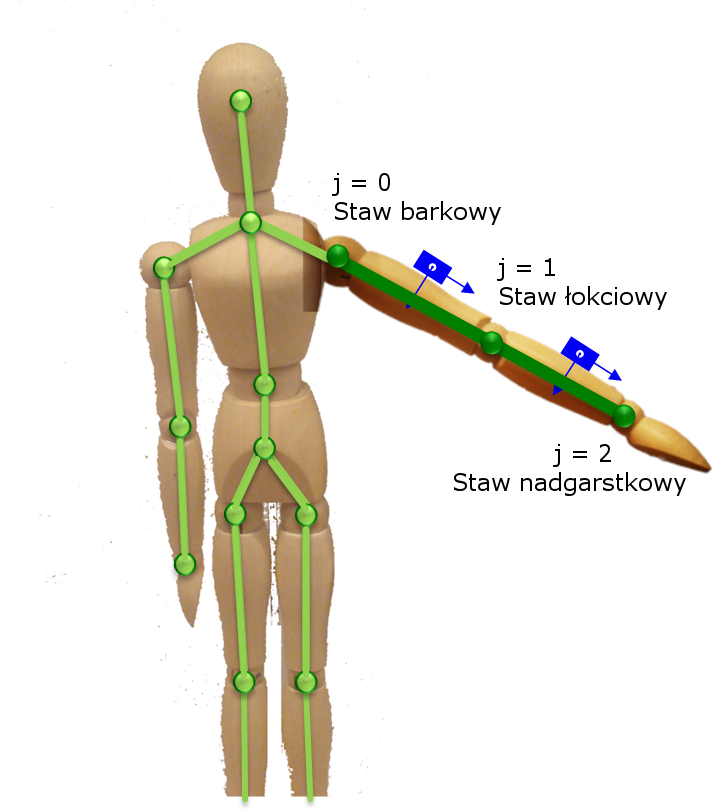
\includegraphics[width=0.75\textwidth]{images/joints.png}
	\caption{Przykład hierarchii stawów dla modelu szkieletowego ręki (źródło: opracowanie własne)}		
	\label{fig:hybrid:jointsHierarchy}		
\end{figure}

		
Zadaniem, omawianej w~niniejszym rozdziale, hybrydowej metody śledzenia ruchu człowieka jest oszacowanie w~chwili czasu $t$ położenia wybranego stawu $j$ szkieletu postaci ($P^F_{j,t} = [p^F_{j,x}, p^F_{j,y}, p^F_{j,z}]_t$, $F$ -- \emph{ang. Fused})  w~przestrzeni trójwymiarowej opisanej w~referencyjnym układzie współrzędnych $X Y Z$, tożsamym z~układem współrzędnych kontrolera Kinect. W~zakresie pojedynczego modułu inercyjnego szacowanie położenia stawu odbywa się na podstawie pomiaru sił działających na akcelerometr w~każdej z~trzech osi ($A = [a_x, a_y, a_z]$), pomiaru prędkości kątowych, z~jakimi porusza się żyroskop względem każdej z~osi ($G = [g_x, g_y, g_z]$) oraz aktualnej temperatury pracy czujników inercyjnych ($T$). Pomiary uzyskane z~akcelerometru oraz żyroskopu wyrażone są w~układzie współrzędnych modułu inercyjnego (rys.~\ref{fig:characteristics:imu:space}). W~przypadku kontrolera Kinect pobierane są pozycje dwóch stawów: stawu $j$, którego pozycja będzie szacowana ($P^K_{j} = [p^K_{j,x}, p^K_{j,y}, p^K_{j,z}]$, $K$--Kinect) oraz stawu $j-1$ ($P^K_{j-1} = [p^K_{j-1,x},p^K_{j-1,y}, p^K_{j-1,z}]$), będącego jego rodzicem w~modelu szkieletowym Kinecta (rys.~\ref{fig:hybrid:jointsHierarchy}). Fuzja danych z~czujników inercyjnych ($A$~oraz $G$) oraz z~kontrolera Kinecta ($P^K_j$) pozwala oszacować pozycję stawu $j$ w~danej chwili $t$ ($P^F_{j,t}$) i~odbywa się z~pewnym interwałem czasowym $\Delta t$, określającym czas pomiędzy kolejnymi aktualizacjami pomiarów kontrolera Kinect, a~będącym jednocześnie interwałem czasowym dla procesu decymacji sygnału urządzeń inercyjnych. Dodatkowymi parametrami wykorzystywanymi w~procesie łączenia danych z~modułu inercyjnego z~pomiarami Kinecta są pozycje obu stawów barkowych uzyskane za pomocą kontrolera Kinect ($P^K_{sh_L,t}, P^K_{sh_R,t}$). Pozwalają one oszacować:

\begin{enumerate}
	\item jak śledzona postać jest obrócona względem Kinecta,
	\item pozycję stawu rodzica ($P^F_{j-1,t}$) w~globalnym układzie współrzędnych, będącą wynikiem osobnej fuzji danych,
	\item długość kości $l$, na której umieszczony jest moduł inercyjny.
\end{enumerate}

Biorąc pod uwagę powyższe, oszacowanie pozycji wybranego stawu $j$, w~hybrydowej metodzie śledzenia ruchu człowieka, można wyrazić za pomocą uogólnionego wzoru \ref{eq:methodFormula}, którego szczegółowy kształt zostanie przedstawiony w~dalszej części pracy.
		
\begin{equation}
	P^F_{j,t} = [p_{j,x}^F,p_{j,y}^F,p_{j,z}^F]_t = f(A,G,T,P_{j-1,t}^K,P_{j,t}^K,\Delta t, P^F_{j-1,t}, P^K_{sh_L,t},P^K_{sh_R,t},l) 
	\label{eq:methodFormula}
\end{equation}
%A - akcelerometr - potrzebny do madgwicka
%G - żyroskop - potrzebny do madgwicka
%T - temperatura - potrzebna do korekty akcelerometru
%P_j^K - staw śledzony pobrany z~Kinecta, potrzebny do fuzji
%P_j-1^K - staw rodzica pobrany z~kinecta
%P^F_{j-1,t} - staw rodzica już po fuzji. względem niego będzie wyrównany punkt wynikowy
% \Delta t - różnica czasu pomiędzy kolejnymi łączeniami dla filtru madgwicka
%------
%l - długość wybranej kości żeby wyznaczyć położenie stawu po fuzji
%P_shR^K, P_shL^K - położenie stawów barkowych z~kinecta do obliczenia orientacji względem kamery 
		
		
Wzór \ref{eq:methodFormula} odnosi się do każdego modułu inercyjnego zbudowanego z~pary czujników: akcelerometru i~żyroskopu, umieszczonego na ciele pomiędzy dwoma kolejnymi stawami, których pozycje oszacowane przez kontroler Kinect są argumentami metody. W~przypadku śledzenia ruchu więcej niż jednego stawu, powyższą metodę należy wykonać zgodnie z~ustaloną hierarchią stawów rozpoczynając od przyjętego korzenia. Oszacowana, w~wyniku fuzji, pozycja stawu $P^F_{j,t}$ określa jego położenie w~globalnym układzie współrzędnych prezentowanego systemu śledzenia ruchu, który pokrywa się z~układem współrzędnych kontrolera Kinect.
		
\section{Format danych używany przez urządzenia pomiarowe}
\subsection{Kontroler Kinect}
Kontroler Kinect w~ramach pakietu pomiarów, rejestrowanego z~częstotliwością $30 Hz$, udostępnia 3 kategorie danych dotyczących obserwowanej sceny: obraz z~kamery RGB, mapę głębi sceny oraz model szkieletowy postaci widocznej na scenie. Kontroler Kinect może jednocześnie zrekonstruować modele szkieletowe dwóch postaci i~śledzić ich kolejne pozy, rejestrując tym samym ich ruch. W~zależności od potrzeb, aplikacja wykorzystująca kontroler Kinect może uzyskać wszystkie 3 kategorie danych jednocześnie lub wybrać tylko te z~nich, które potrzebuje do swojego działania. Opisywana w~niniejszej dysertacji hybrydowa metoda śledzenia ruchu kończyn człowieka bazuje na informacji dotyczącej modelu szkieletowego śledzonej postaci wybierając z~pełnego modelu tylko informacje związane z~wybranymi stawami reprezentującymi śledzoną kończynę oraz te, na podstawie których można określić wiarygodność pomiarów uzyskanych za pomocą kontrolera Kinect. Na przykład przy śledzeniu ruchu prawej ręki są to oba stawy barkowe, prawy staw łokciowy oraz prawy staw nadgarstkowy. Każdy staw $j$ reprezentowany jest przez trzy współrzędne ($P^K_j = [p^K_{j,x}, p^K_{j,y}, p^K_{j,z}]$) określające jego położenie w~przestrzeni w~układzie współrzędnych kontrolera Kinect oraz informacje o~stanie śledzenia tego stawu: \emph{Tracked}, \emph{Interferred} albo \emph{NotTracked}. Na podstawie współrzędnych stawów barkowych postaci obliczany jest kąt obrotu sylwetki względem Kinecta (wzór \ref{eq:characteristics:kinect:bodyRotationAngle}). Dodatkowo każdy pakiet danych zawiera informacje o~swoim numerze, znacznik czasu wygenerowany przez kontroler Kinect oraz godzinę odebrania danych na komputerze, do którego podłączone jest to urządzenie.
		
\subsection{Czujniki inercyjne}
Moduły inercyjne (IMU1 i~IMU2) zbudowane zostały z~czujników inercyjnych: akcelerometru i~żyroskopu, podłączonych bezpośrednio do jednostki centralnej opartej na platformie Arduino. Częstotliwość odczytu danych z~czujników kontrolowana jest przez zewnętrzny moduł zegara (RTC DS3230), który również został podłączony bezpośrednio do Arduino{\footnote{Arduino -- platforma programistyczna dla systemów wbudowanych, \url{www.arduino.cc}}}. Zadaniem jednostki centralnej jest odczyt danych z~czujników, sformatowanie ich i~wysłanie z~wykorzystaniem technologii Bluetooth (BT HC-05) do komputera PC, gdzie następuje dalsze ich przetwarzanie (uproszczony schemat urządzenia do pomiaru danych inercyjnych\footnote{Urządzenie do pomiaru danych inercyjnych jest urządzeniem zaprojektowanym i~wykonanym przez autora niniejszej dysertacji.} przedstawia rys.~\ref{fig:device:circuitDiagram}). Odczyt pakietu danych z~pojedynczego modułu obejmuje:

\begin{enumerate}
	\item zestaw pomiarów udostępnionych przez żyroskop (trzy wartości obrotu $G = [g_x, g_y, g_z]$, po jednej dla każdej z~osi),
	\item zestaw pomiarów z~akcelerometru (trzy wartości przyspieszenia $A = [a_x, a_y, a_z]$),
	\item pomiar temperatury czujników $T$.
\end{enumerate}

Wszystkie pomiary przesyłane są jako 16-bitowe liczby całkowite ze znakiem i~pomiary ze wszystkich podłączonych modułów wysyłane są do komputera PC jednocześnie. Przesyłane wartości muszą być następnie skonwertowane do jednostek odpowiadających wielkościom fizycznym mierzonym przez poszczególne czujniki. Dla żyroskopu są to stopnie na sekundę ($\degree/s$), dla akcelerometru -- jednostki przyspieszenia grawitacyjnego ($g$), które można również przeliczyć na jednostki przyspieszenia $m/_{s^2}$, a~dla temperatury stopnie Celsjusza ($\degree C$). W~przypadku danych z~czujników inercyjnych konwersja polega na podzieleniu wartości bezpośredniego odczytu z~czujników przez współczynniki odpowiednie dla zakresu pracy tych czujników. Tabele \ref{tab:hybrid:accRangeFactors} oraz \ref{tab:hybrid:gyroRangeFactors} przedstawiają zestawienie współczynników konwersji $f_A$ i~$f_G$ wykorzystywanych do konwersji pomiarów odpowiednio z~akcelerometru i~żyroskopu. Jak już zostało to zaznaczone wcześniej, w~trakcie prowadzonych eksperymentów badawczych, zakres pracy akcelerometru został ustalony na $\pm4g$, natomiast żyroskopu na $\pm500\degree/s$. Jako zakresy pracy czujników modułów inercyjnych przyjęto podobne wartości do tych zastosowanych w~kontrolerze ruchu Nintendo Wii Remote Plus. 
	
\begin{figure}[!htb]
		\captionsetup{singlelinecheck=off}
	\centering
	\rotatebox{-90}{
		\begin{figure}[!htp]
	\centering
	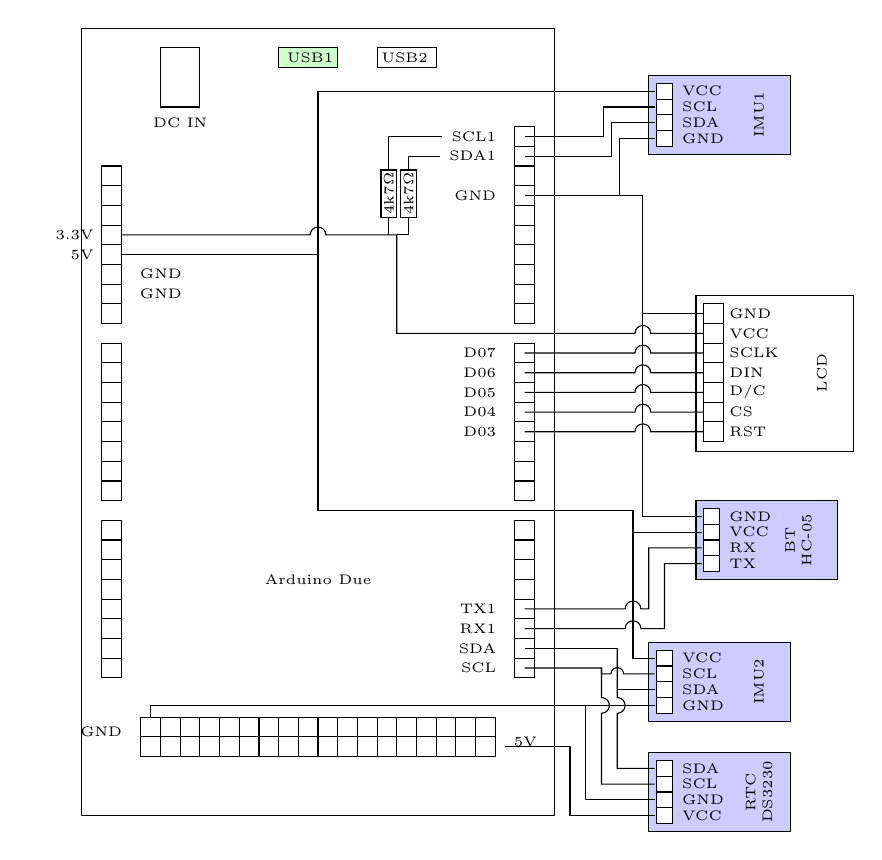
\begin{tikzpicture}
		\draw  (-3,5) rectangle (3,-5); % board
		\draw  (-2,4.75) rectangle (-1.5,4); % DC in
		\node [font=\tiny]   at(-1.75, 3.8){DC IN};
		\draw[fill=green!20]  (-0.5,4.75) rectangle (0.25,4.5); % USB 1
		\node [font=\tiny]   at(-0.1, 4.62){USB1};
		\draw  (0.75,4.75) rectangle (1.5,4.5); % USB 2
		\node [font=\tiny]   at(1.1, 4.62){USB2};
		\draw (2.5,3.75) rectangle (2.75,1.25);%SCL1
		\draw (2.5,3.5) -- (2.75, 3.5);%SDA1
		\draw (2.5,3.25) -- (2.75, 3.25);%AREF
		\draw (2.5,3) -- (2.75, 3);%GND
		\draw (2.5,2.75) -- (2.75, 2.75);%D13
		\draw (2.5,2.5) -- (2.75, 2.5);%D12
		\draw (2.5,2.25) -- (2.75, 2.25);%D11
		\draw (2.5,2) -- (2.75, 2);%D10
		\draw (2.5,1.75) -- (2.75, 1.75);%D09
		\draw (2.5,1.5) -- (2.75, 1.5);%D08
		\draw  (2.5,1) rectangle (2.75,-1);%D07
		\draw (2.5,0.75) -- (2.75, 0.75);%D06
		\draw (2.5,0.5) -- (2.75, 0.5);%D05
		\draw (2.5,0.25) -- (2.75, 0.25);%D04
		\draw (2.5,0) -- (2.75, 0);%D03
		\draw (2.5,-0.25) -- (2.75, -0.25);%D02
		\draw (2.5,-0.5) -- (2.75, -0.5); %TX0 -> 1
		\draw (2.5,-0.75) -- (2.75, -0.75); %RX0 -> 2
		\draw  (2.5,-1.25) rectangle (2.75,-3.25); %TX3
		\draw (2.5,-1.5) -- (2.75, -1.5); %RX3
		\draw (2.5,-1.75) -- (2.75, -1.75); %TX2
		\draw (2.5,-2) -- (2.75, -2); %RX2
		\draw (2.5,-2.25) -- (2.75, -2.25); %TX1
		\draw (2.5,-2.5) -- (2.75, -2.5); %RX1
		\draw (2.5,-2.75) -- (2.75, -2.75); %SDA
		\draw (2.5,-3) -- (2.75, -3); %SCL
		\draw  (-2.75,3.25) rectangle (-2.5,1.25);
		\draw (-2.75,3) -- (-2.5, 3);%IOREF
		\draw (-2.75,2.75) -- (-2.5, 2.75);%RESET
		\draw (-2.75,2.5) -- (-2.5, 2.5);%3.3V
		\draw (-2.75,2.25) -- (-2.5, 2.25);%5V
		\draw (-2.75,2) -- (-2.5, 2);%GND
		\draw (-2.75,1.75) -- (-2.5, 1.75);%GND
		\draw (-2.75,1.5) -- (-2.5, 1.5);%VIN
		\draw  (-2.75,1) rectangle (-2.5,-1); %A0
		\draw (-2.75,0.75) -- (-2.5, 0.75);%A1
		\draw (-2.75,0.5) -- (-2.5, 0.5);%A2
		\draw (-2.75,0.25) -- (-2.5, 0.25);%A3
		\draw (-2.75,0) -- (-2.5, 0);%A4
		\draw (-2.75,-0.25) -- (-2.5, -0.25);%A5
		\draw (-2.75,-0.5) -- (-2.5, -0.5); %A6
		\draw (-2.75,-0.75) -- (-2.5, -0.75); %A7
		\draw  (-2.75,-1.25) rectangle (-2.5,-3.25);%A08
		\draw (-2.75,-1.5) -- (-2.5, -1.5); %TX0 -> 1
		\draw (-2.75,-1.75) -- (-2.5, -1.75); %RX0 -> 2
		\draw (-2.75,-2) -- (-2.5, -2);%A4
		\draw (-2.75,-2.25) -- (-2.5, -2.25);%A5
		\draw (-2.75,-2.5) -- (-2.5, -2.5); %A6
		\draw (-2.75,-2.75) -- (-2.5, -2.75); %A7
		\draw (-2.75,-3) -- (-2.5, -3);%A4
		\draw  (-2.25,-3.75) rectangle (2.25,-4.25);
		\draw  (-2.25,-4) -- (2.25,-4);
		\draw  (-2,-3.75) -- (-2,-4.25);
		\draw  (-1.75,-3.75) -- (-1.75,-4.25);
		\draw  (-1.5,-3.75) -- (-1.5,-4.25);
		\draw  (-1.25,-3.75) -- (-1.25,-4.25);
		\draw  (-1,-3.75) -- (-1,-4.25);
		\draw  (-0.75,-3.75) -- (-0.75,-4.25);
		\draw  (-0.5,-3.75) -- (-0.5,-4.25);
		\draw  (-0.25,-3.75) -- (-0.25,-4.25);
		\draw  (0,-3.75) -- (0,-4.25);
		\draw  (0.25,-3.75) -- (0.25,-4.25);
		\draw  (0.5,-3.75) -- (0.5,-4.25);
		\draw  (0.75,-3.75) -- (0.75,-4.25);
		\draw  (1,-3.75) -- (1,-4.25);
		\draw  (1.25,-3.75) -- (1.25,-4.25);
		\draw  (1.5,-3.75) -- (1.5,-4.25);
		\draw  (1.75,-3.75) -- (1.75,-4.25);
		\draw  (2,-3.75) -- (2,-4.25);
		%IMU1
		\draw  [fill=blue!20](4.2,4.4) rectangle (6,3.4);
		\draw  [fill=white](4.3,4.3) rectangle (4.5,3.5);
		\draw  (4.3,4.1) -- (4.5,4.1);
		\draw  (4.3,3.9) -- (4.5,3.9);
		\draw  (4.3,3.7) -- (4.5,3.7);
		%IMU2
		\draw  [fill=blue!20](4.2,-2.8) rectangle (6,-3.8);
		\draw  [fill=white](4.3,-2.9) rectangle (4.5,-3.7);
		\draw  (4.3,-3.1) -- (4.5,-3.1);
		\draw  (4.3,-3.3) -- (4.5,-3.3);
		\draw  (4.3,-3.5) -- (4.5,-3.5);
		%BT
		\draw  [fill=blue!20](4.8,-1) rectangle (6.6,-2);
		\draw  [fill=white](4.9,-1.1) rectangle (5.1,-1.9);
		\draw  (4.9,-1.3) -- (5.1,-1.3);
		\draw  (4.9,-1.5) -- (5.1,-1.5);
		\draw  (4.9,-1.7) -- (5.1,-1.7);
		%RTC
		\draw  [fill=blue!20](4.2,-4.2) rectangle (6,-5.2);
		\draw  [fill=white](4.3,-4.3) rectangle (4.5,-5.1);
		\draw  (4.3,-4.5) -- (4.5,-4.5);
		\draw  (4.3,-4.7) -- (4.5,-4.7);
		\draw  (4.3,-4.9) -- (4.5,-4.9);
		%LCD
		\draw  (4.8,1.6) rectangle (6.8,-0.375);
		\draw  (4.9,1.5) rectangle (5.15,-0.25);
		\draw (4.9,1.25) -- (5.15, 1.25); 
		\draw (4.9,1) -- (5.15, 1); 
		\draw (4.9,0.75) -- (5.15, 0.75);
		\draw (4.9,0.5) -- (5.15, 0.5);
		\draw (4.9,0.25) -- (5.15, 0.25);
		\draw (4.9,0) -- (5.15, 0);
		\node[left, font=\tiny] (SCL1) at (2.625,3.625) {SCL1$\quad$};
		\node[left, font=\tiny] (SDA1) at (2.625,3.375) {SDA1$\quad$};
		\node[left, font=\tiny] (GND) at (2.625,2.875) {GND$\quad$};
		\node[left, font=\tiny] (D07) at (2.625,0.875) {D07$\quad$};
		\node[left, font=\tiny]  (D06) at (2.625,0.625) {D06$\quad$};
		\node[left, font=\tiny]  (D05) at (2.625,0.375) {D05$\quad$};
		\node[left, font=\tiny]  (D04) at (2.625,0.125) {D04$\quad$};
		\node[left, font=\tiny]  (D03) at (2.625,-0.125) {D03$\quad$};
		\node[left, font=\tiny]  (TX1) at (2.625,-2.375) {TX1$\quad$};
		\node[left, font=\tiny]  (RX1) at (2.625,-2.625) {RX1$\quad$};
		\node[left, font=\tiny]  (SDA) at (2.625,-2.875) {SDA$\quad$};
		\node[left, font=\tiny]  (SCL) at (2.625,-3.125) {SCL$\quad$};
		\node (GND3) at (-2.125,-3.875) {};
		\node[above left, font=\tiny] (GND4) at (-2.125,-4.125) {GND$\quad$};
		\node[below right, font=\tiny] (50V3) at (2.125,-3.875) {$\quad$5V};
		\node[right, font=\tiny] (50V4) at (2.125,-4.125) {};
		\node (33V)at (-2.625,2.375) {};
		\node[left, font=\tiny] at (-2.725,2.375) {$\quad$3.3V};
		\node (50V) at (-2.625,2.125) {};
		\node[left, font=\tiny]  at (-2.725,2.125) {$\quad$5V};
		\node[right, font=\tiny]  (GND1) at (-2.625,1.875) {$\quad$GND};
		\node[right, font=\tiny]  (GND2) at (-2.625,1.625) {$\quad$GND};
		\node(IMU1VCC) at (4.4,4.2) {};
		\node(IMU1SCL) at (4.4,4.0) {};
		\node(IMU1SDA) at (4.4,3.8) {};
		\node(IMU1GND) at (4.4,3.6) {};
		\node[right, font=\tiny] at (4.5,4.2) {VCC};
		\node[right, font=\tiny] at (4.5,4) {SCL};
		\node[right, font=\tiny] at (4.5,3.8) {SDA};
		\node[right, font=\tiny] at (4.5,3.6) {GND};
		\node[rotate=90, font=\tiny] at (5.6,3.9) {IMU1};
		\node(IMU2VCC) at (4.4,-3) {};
		\node(IMU2SCL) at (4.4,-3.2) {};
		\node(IMU2SDA) at (4.4,-3.4) {};
		\node(IMU2GND) at (4.4,-3.6) {};
		\node[right, font=\tiny] at (4.5,-3) {VCC};
		\node[right, font=\tiny] at (4.5,-3.2) {SCL};
		\node[right, font=\tiny] at (4.5,-3.4) {SDA};
		\node[right, font=\tiny] at (4.5,-3.6) {GND};
		\node[rotate=90, font=\tiny] at (5.6,-3.3) {IMU2};
		\node(BTGND) at (5,-1.2) {};
		\node(BTVCC) at (5,-1.4) {};
		\node(BTRX) at (5,-1.6) {};
		\node(BTTX) at (5,-1.8) {};
		\node[right, font=\tiny] at (5.1,-1.2) {GND};
		\node[right, font=\tiny] at (5.1,-1.4) {VCC};
		\node[right, font=\tiny] at (5.1,-1.6) {RX};
		\node[right, font=\tiny] at (5.1,-1.8) {TX};
		\node[rotate=90, font=\tiny, align=center] at (6.1,-1.5) {BT \\ HC-05};
		\node(RTCSDA) at (4.4,-4.4) {};
		\node(RTCSCL) at (4.4,-4.6) {};
		\node(RTCGND) at (4.4,-4.8) {};
		\node(RTCVCC) at (4.4,-5) {};
		\node[right, font=\tiny] at (4.5,-4.4) {SDA};
		\node[right, font=\tiny] at (4.5,-4.6) {SCL};
		\node[right, font=\tiny] at (4.5,-4.8) {GND};
		\node[right, font=\tiny] at (4.5,-5) {VCC};
		\node[rotate=90, font=\tiny, align=center] at (5.6,-4.7) {RTC \\ DS3230};
		\node (LCDGND) at (5.025,1.375) {};
		\node (LCDVCC) at (5.025,1.125) {};
		\node (LCDD07) at (5.025,0.875) {};
		\node (LCDD06) at (5.025,0.625) {};
		\node (LCDD05) at (5.025,0.375) {};
		\node (LCDD04) at (5.025,0.125) {};
		\node (LCDD03) at (5.025,-0.125) {};
		\node[right, font=\tiny] at (5.1,1.375) {GND};
		\node[right, font=\tiny] at (5.1,1.125) {VCC};
		\node[right, font=\tiny] at (5.1,0.875) {SCLK};
		\node[right, font=\tiny] at (5.1,0.625) {DIN};
		\node[right, font=\tiny] at (5.1,0.375) {D/C};
		\node[right, font=\tiny] at (5.1,0.125) {CS};
		\node[right, font=\tiny] at (5.1,-0.125) {RST};
		\node[rotate=90, font=\tiny, align=center] at (6.4,0.625) {LCD};
		\draw(SCL1) --(3.625,3.625) |- (IMU1SCL);
		\draw  (SDA1)--(3.725,3.375)  |-(IMU1SDA);
		\draw  (GND) -- (3.825,2.875)|- (IMU1GND);
		\draw  (50V) --(0,2.125) |- (IMU1VCC);
		\draw  (50V) --(0,2.125)--(0,-1.125)--(4,-1.125) |- (IMU2VCC);
		\draw (SDA) -- (3.8,-2.875) |-(IMU2SDA);
		\draw(SCL) -- (3.6,-3.125) |- (3.72,-3.2) arc(180:0:0.08)--(IMU2SCL);4.4,-3.2
		\draw (GND3) |- (IMU2GND);
		\draw(4,-1.125) |- (BTVCC);
		\draw(TX1) --(3.9,-2.375) arc(180:0:0.1)--(4.2,-2.375) |-(BTRX);
		\draw(RX1) --(3.9,-2.625) arc(180:0:0.1)--(4.4,-2.625) |-(BTTX);
		\draw  (GND) -- (4.125,2.875)|- (BTGND);
		\draw  (4.125,1.375) -- (LCDGND);
		\draw (33V) -- (-0.1,2.375) arc(180:0:0.1)-- (1,2.375) |-(4.025,1.125) arc(180:0:0.1)-- (LCDVCC);
		\draw (D07) --(4.025,0.875) arc(180:0:0.1)-- (LCDD07);
		\draw (D06) --(4.025,0.625) arc(180:0:0.1)-- (LCDD06);
		\draw (D05) --(4.025,0.375) arc(180:0:0.1)--(LCDD05);
		\draw (D04) --(4.025,0.125) arc(180:0:0.1)-- (LCDD04);
		\draw (D03) --(4.025,-0.125) arc(180:0:0.1)-- (LCDD03);
		\draw(3.8,-2.875) --(3.8,-3.5) arc(90:-90:0.1)|-(RTCSDA);
		\draw(3.6,-3.125)--(3.6,-3.5) arc(90:-90:0.1) |-(RTCSCL);
		\draw(3.4,-3.6) |-(RTCGND);
		\draw(50V4) -- (3.2, -4.125) |- (RTCVCC);
		\draw(0.9,2.375)--(0.9,2.6);
		\draw(1,2.375)-|(1.15,2.6);
		\draw(0.9,3.2)|-(SCL1);
		\draw(1.15,3.2) |-(SDA1);
		\draw  (1.05,3.2) rectangle (1.25,2.6);
		\draw  (0.8,3.2) rectangle (1.,2.6);
		\node[font=\tiny, rotate=90] at (0.9,2.9) {4k7$\Omega$};
		\node[font=\tiny, rotate=90] at (1.15,2.9) {4k7$\Omega$};
		\node[font=\tiny] at (0,-2) {Arduino Due};
	\end{tikzpicture}
	\caption{Schemat budowy urządzenia pomiarowego opartego o~komputer Arduino.}
													
	\label{fig:device:circuitDiagram}
\end{figure}
	}
	\caption{Schemat budowy urządzenia pomiarowego opartego o~komputer Arduino (źródło: badania własne). IMU1 i~IMU2 -- Moduły inercyjne, RTC -- moduł zagara oparty o~komponent DS3230, BT -- moduł Bluetooth oparty o~komponent HC-05, LCD -- ekran ciekłokrystaliczny}	
	\label{fig:device:circuitDiagram}
\end{figure}
		
\begin{savenotes}
	\begin{table}[!htb]
		\caption[Współczynniki konwersji bezpośrednich pomiarów akcelerometru (a) i~żyroskopu (b) w~zależności od przyjętego zakresu pracy]{Współczynniki konwersji bezpośrednich pomiarów akcelerometru (a) i~żyroskopu (b) w~zależności od przyjętego zakresu pracy\footfullcite{footnote:ivenSense:MPU6050}}
		\begin{subtable}{.5\linewidth}
			\centering
			\caption{Akcelerometr}
			\label{tab:hybrid:accRangeFactors} 
			\begin{tabular}{|l|c|}
				\hline
				Zakres pomiaru              & Współczynnik \\ \hline
				$\pm2g$                     & $16384$        \\ \hline
				\rowcolor{black!20} $\pm4g$ & $8192$         \\ \hline
				$\pm8g$                     & $4096$         \\ \hline
				$\pm16g$                    & $2048$         \\ \hline
			\end{tabular}
		\end{subtable}%
		\begin{subtable}{.5\linewidth}
			\centering
			\caption{Żyroskop}
			\label{tab:hybrid:gyroRangeFactors}	
			\begin{tabular}{|l|c|}
				\hline
				Zakres pomiaru                        & Współczynnik \\ \hline
				$\pm250\frac{\degree}{s}$             & $131.0$        \\ \hline
				\rowcolor{black!20} $\pm500\degree/s$ & $65.5$         \\ \hline
				$\pm1000\frac{\degree}{s}$            & $32.8$         \\ \hline
				$\pm2000\frac{\degree}{s}$            & $16.4$         \\ \hline
			\end{tabular}
		\end{subtable} 
	\end{table}
\end{savenotes}	
		
		
Konwersja pomiaru temperatury czujników ($T_{raw}$) do wartości wyrażonej w~$\degree C$ ($T_{deg}$) wymaga zastosowania wzoru \ref{eq:hybrid:tempEquation}

\begin{equation}
	T_{deg} = 36.53 + T_{raw} / 340.0
	\label{eq:hybrid:tempEquation}
\end{equation}

wynikającego ze specyfikacji zastosowanego układu elektronicznego IvenSense MPU-6050. Wartości stałe zastosowane w~tym wzorze związane są z~rozdzielczością pomiarów wykorzystanego w~tym układzie elektronicznym termometru (wartość = 340.0) oraz ze stałego przesunięcia dla temperatury $0 \degree C$ (wartość = 36.53)
				
Do danych pobranych ze wszystkich podłączonych modułów inercyjnych, podobnie jak w~przypadku danych z~Kinecta, dołączone są znaczniki czasowe zarówno ustawiane przez urządzenie, jak i~przez komputer PC w~momencie odbioru danych oraz numeracja kolejnych pakietów danych. Odczyt danych z~modułów inercyjnych odbywa się z~częstotliwością $100Hz$.
		
\section{Kalibracja}
W proponowanym systemie czujniki inercyjne wymagają kalibracji przy każdym uruchomieniu. Kalibracja Kinecta nie jest wymagana, a~jedyne co należy zrobić to upewnić się, że kąt nachylenia kamery pozwala na obserwację śledzonej postaci.
		
Kalibracja czujników inercyjnych przebiega dwuetapowo w~następującej kolejności:
\begin{enumerate}
	\item {Wyznaczenie współczynników korekty odchylenia pomiarów czujników inercyjnych dla wartości spoczynkowych.} 
	\item {Inicjalizacja filtru Madgwicka wyznaczającego orientację sensora na podstawie danych z~czujników inercyjnych.}
\end{enumerate}
		
Krok pierwszy służy do wyznaczenia macierzy współczynników korekty ($cor = [cor_A \quad cor_G]^T = [[c_{AX},c_{AY},c_{AZ}]\quad [c_{GX},c_{GY},c_{GZ}]]^T $) pomiarów spoczynkowych ($G, A$) dla każdego modułu inercyjnego indywidualnie. W~trakcie tego kroku kalibrowane czujniki należy umieścić możliwie jak najbardziej poziomo tak, żeby oś $Z$ sensora była równoległa do kierunku działania siły grawitacji. Dla czujników znajdujących się w~takim właśnie położeniu można określić jakich wartości pomiarów należy oczekiwać ($A_0 = [0,0,1]$ dla akcelerometru oraz $G_0 = [0,0,0]$ dla żyroskopu). W~praktyce jednak, ze względu na zaszumienie danych i~brak możliwości całkowitego ich oczyszczenia, wartości idealne nie są osiągalne. W~związku z~tym, algorytm odpowiedzialny za kalibrację działa iteracyjnie ($s$ -- indeks iteracji) tak długo, dopóki jakikolwiek element macierzy średnich błędów pomiarów czujników inercyjnych ($[\overline{A}\quad \overline{G}]^T = [[\overline{a_x},\overline{a_y},\overline{a_z}]\quad[\overline{g_x},\overline{g_y},\overline{g_z}]]^T$ jest większy od elementu o~tym samym indeksie w~macierzy akceptowalnych błędów pomiaru ($[A_{th}\quad G_{th}]^T = [[a_{x,th},a_{y,th},a_{z,th}]\quad[g_{x,th},g_{y,th},g_{z,th}]]^T $. Stop następuje, gdy prawdą jest następujący warunek: $[\overline{A}\quad \overline{G}] \leq [A_{th}\quad G_{th}] \Leftrightarrow \overline{a_x}\leq a_{x,th} \land \overline{a_y} \leq a_{y,th} \land \overline{a_z} \leq a_{z,th} \land \overline{g_x} \leq g_{x,th} \land \overline{g_y} \leq g_{y,th} \land \overline{g_z} \leq g_{z,th}$). W~rezultacie elementy macierzy $cor$ pozwalają uzyskać pomiary w~każdej z~osi z~założoną dokładnością. Przyjmując, że macierz $[A_0\quad G_0]$ zawiera oczekiwane wartości pomiarów dla akcelerometru i~żyroskopu, a~$[A\quad G]_{s,i}$ to $i$-ty z~$n$ kolejnych pomiarów obu czujników dla iteracji $s$, średnie błędy pomiarów wyznaczone są zgodnie ze wzorem \ref{eq:hybrid:IMUCalibration:1}.
\begin{equation}
	\begin{bmatrix} \overline{A} \\ \overline{G} \end{bmatrix}_s =
	\begin{cases}
		\frac{1}{n}\sum_{i=1}^{n}{\begin{bmatrix}A \\ G\end{bmatrix}_{s,i}} & s = 1\\
		\frac{1}{n}\sum_{i=1}^{n}{\begin{bmatrix}A \\ G\end{bmatrix}_{s,i} - \begin{bmatrix}cor_A\\ cor_G\end{bmatrix}_{s-1}} &  s > 1
	\end{cases}
	\label{eq:hybrid:IMUCalibration:1}
\end{equation}

natomiast macierz współczynników korekty $cor$ wyznaczona jest na podstawie wzoru \ref{eq:hybrid:IMUCalibration:2}.

\begin{equation}
	\begin{split}
		&cor_s = \begin{bmatrix}cor_A\\ cor_G\end{bmatrix}_s = \begin{bmatrix}c_{AX} & c_{AY} & c_{AZ} \\ c_{GX} & c_{GY} & c_{GZ}\end{bmatrix}_s = \\
		&\begin{cases}
		\frac{1}{8}\left(\begin{bmatrix}A_0 \\ G_0\end{bmatrix} - \begin{bmatrix}\overline{A}\\ \overline{G}\end{bmatrix}_1\right) & s = 1\\
		cor_{s-1} - diag(\frac{1}{a_{x,th}},\frac{1}{a_{y,th}},\frac{1}{a_{z,th}},\frac{1}{g_{x,th}},\frac{1}{g_{y,th}},\frac{1}{g_{z,th}}) 
		\left(\begin{bmatrix}A_0 \\ G_0\end{bmatrix} - \begin{bmatrix}\overline{A}\\ \overline{G}\end{bmatrix}_n\right) & s > 1
		\end{cases}
	\end{split}
	\label{eq:hybrid:IMUCalibration:2}
\end{equation}

Wyznaczone w~ten sposób współczynniki korekty: $c_{AX}$, $c_{AY}$, $c_{AZ}$, $c_{GX}$, $c_{GY}$, $c_{GZ}$ wykorzystywane są następnie do ciągłej korekty pomiarów uzyskiwanych z~akcelerometrów i~żyroskopów. Kalibracja modułu zajmuje zwykle około 10 iteracji, natomiast zdarzały się sytuacje, w~których trwało to ponad 2 razy dłużej. Było to zazwyczaj spowodowane poruszeniem modułu w~trakcie kalibracji. Schemat na rysunku \ref{fig:hybrid:IMUCalibration} przedstawia schemat blokowy procedury kalibracji czujników inercyjnych.

\begin{figure}[!htb]
	\scalebox{0.55}{		
		\begin{tikzpicture} [	
		node distance=1cm,
		start/.style = {ellipse,fill=red!30, minimum height=2em},
		decision/.style = { diamond, draw=black, thick, fill=black!5, text width=6em, text badly centered, inner sep=1pt, rounded corners },
		block/.style    = { rectangle, draw=black, thick, fill=black!5, text width=26em, text centered, rounded corners, minimum height=2em },
		line/.style     = { draw, thick, ->, shorten >=2pt },
		action/.style = {trapezium, draw=black, thick, fill=black!5,  text width=16em, text centered, trapezium left angle=-100, trapezium right angle=-80}
	]
	% Define nodes in a~matrix
	\begin{scope}
		\node [start] (start) {Start};\\
		\node [block, below=of start] (init) {$s:=1 \quad\quad n:=1000$ \\        			
			$cor_0 = \begin{bmatrix}cor_A \\ cor_G\end{bmatrix}_0 := \begin{bmatrix}0, 0, 0 \\ 0, 0, 0\end{bmatrix} \quad\quad \begin{bmatrix}A_0 \\ G_0 \end{bmatrix} := \begin{bmatrix}0,0,1 \\ 0,0,0\end{bmatrix}$ \\
			$\begin{bmatrix} A_{th} \\ G_{th}\end{bmatrix} := \begin{bmatrix}a_{x,th},a_{y,th},a_{z,th}\\ g_{x,th},g_{y,th},g_{z,th}\end{bmatrix} \quad\quad \begin{bmatrix} A \\ G\end{bmatrix} := \begin{bmatrix}a_{x},a_{y},a_{z}\\ g_{x},g_{y},g_{z}\end{bmatrix}$ \\    
			};\\
																		
		\node [block, below=of init] (resetCounter) {$i:=0$\\
			$temp := \begin{bmatrix}0, 0, 0 \\ 0, 0, 0\end{bmatrix}$ \\
			$\begin{bmatrix}\overline{A}\\ \overline{G}\end{bmatrix} = \begin{bmatrix}\overline{a_x},\overline{a_y},\overline{a_z} \\ \overline{g_x},\overline{g_y},\overline{g_z}\end{bmatrix} := \begin{bmatrix}0, 0, 0 \\ 0, 0, 0\end{bmatrix}$};\\
		\node [above=of resetCounter, below, yshift=-0.5cm](nullResetCounter) {};  \\
																		
		\node [decision, below=of resetCounter] (loop1) {$i<n$?}; \\
		\node [above=of loop1, below, yshift=-0.5cm](nullLoop1) {};  \\
																
		\node [left=of loop1,xshift=-3cm] (nullReadMotionData) {};
		\node [action, below=of nullReadMotionData] (readMotionData){$\begin{bmatrix} A \\ G\end{bmatrix} := \begin{bmatrix} odczyt \\ z\quad sensorow\end{bmatrix}- \begin{bmatrix}cor_A\\ cor_G\end{bmatrix}_{s-1}$\\ $temp := temp + \begin{bmatrix} A \\ G\end{bmatrix}$\\$i:=i+1$};  
																		        
		\node [right=of loop1,xshift=3cm] (nullCalculateAverage) {};
		\node [action, below=of nullCalculateAverage] (calculateAverage){$\begin{bmatrix}\overline{A}\\ \overline{G}\end{bmatrix}_s := \frac{1}{n} temp$};\\   
															             
		\node [decision, below=of loop1, yshift=-2cm] (loop2) {
			$\overline{a_x} \leq a_{x,th} \land$\\ 
			$\overline{a_y} \leq a_{y,th} \land$\\ 
			$\overline{a_z} \leq a_{z,th} \land$\\ 
			$\overline{g_x} \leq g_{x,th} \land$\\
			$\overline{g_y} \leq g_{y,th} \land$\\ 
			$\overline{g_z} \leq g_{z,th}$ ?};\\
															
		\node [left=of loop2, xshift=-3cm] (nullReturn){};  
		\node [action, below=of nullReturn] (return){return $cor_s$};  
		\node [start, below=of return] (stop) {Stop};
														
		\node [decision, below=of loop2, yshift=-1cm] (loop3) {$s = 1$?};\\
																
		\node [left=of loop3, xshift=-3cm] (nullCor1) {};
		\node [action, below=of nullCor1] (cor1){$ cor_s =\frac{1}{8}\left(\begin{bmatrix}A_0 \\ G_0\end{bmatrix} - \begin{bmatrix}\overline{A}\\ \overline{G}\end{bmatrix}_s\right)$};
														
		\node [right=of loop3, xshift=4cm] (nullCorS) {};
		\node [action, below=of nullCorS, text width=26em] (corS) {$cor_s = cor_{s-1} +$ \\$ -diag(\frac{1}{a_{x,th}},\frac{1}{a_{y,th}},\frac{1}{a_{z,th}},\frac{1}{g_{x,th}},\frac{1}{g_{y,th}},\frac{1}{g_{z,th}}) \left(\begin{bmatrix}A_0 \\ G_0\end{bmatrix} - \begin{bmatrix}\overline{A}\\ \overline{G}\end{bmatrix}_s\right)$};\\
																		        
		\node [action, below=of loop3, yshift=-2cm] (incS){$s:=s+1$};  \\
	\end{scope}
									
	\begin{scope} [every path/.style=line]
		\path  (start)        --    (init)  --   (resetCounter)   --    (loop1);
		\path  (loop1)  --++  (-3,0) node [near start, above] {Tak} -| (readMotionData)--++ (-4,0) node [near start] {} |-  (nullLoop1);
		\path  (loop1)  --++  (3,0) node [near start, above] {Nie} -| (calculateAverage);	               
		\path  (calculateAverage.south) --++ (0,-1) node {} -| (loop2.north);
		\path (loop2)  --++  (-4,0) node [near start, above] {Tak} -| (return) -- (stop);
		\path (loop2.east) --++  (2,0) node [near start, above] {Nie} --++ (0,-3.5) node {} -| (loop3);
		\path  (loop3)  --++  (-3,0) node [near start, above] {Tak} -| (cor1) --++ (0, -1.5) node(temp) {} -|  (incS.north);
		\path  (loop3)  --++  (3,0) node [near start, above] {Nie} -| (corS) --++  (0, -1.33) node(temp) {} -|  (incS.north);		                 
		\path  (incS.east)  --++  (9.5, 0) node {} |-  (nullResetCounter.east);
	\end{scope}			
\end{tikzpicture}
	}
	\caption{Diagram przedstawiający kalibrację czujników inercyjnych (źródło: badania własne)}
	\label{fig:hybrid:IMUCalibration}
\end{figure}


Kolejnym krokiem jest inicjalizacja filtru Madgwicka łączącego dane z~czujników inercyjnych w~celu wyznaczenia ich orientacji w~przestrzeni. Łączenie to ma na celu ograniczenie dryfu żyroskopu za pomocą pomiarów akcelerometru, a~następnie wyznaczenie orientacji przestrzennej modułu inercyjnego. W~literaturze najczęściej spotykanym filtrem wykorzystywanym do tego celu jest filtr Kalmana \cite{Sasiadek2000, Sabatini2011, Mau2005, Qingming2014} (szczegółowy opis filtrów Kalmana jak i~filtru Madgwicka znajduje się w~dodatku \ref{chap:appx:filters}). W~roku 2010 Sebastian Madgwick opublikował raport ze swoich badań, w~którym przedstawił wzór autorskiego filtru łączącego dane z~akcelerometru i~żyroskopu oraz wariant uzupełniony o~dane z~magnetometru,  przedstawiający orientację urządzenia pomiarowego w~chwili $t$, zbudowanego z~tych czujników, w~postaci kwaternionów \cite{Madgwick2010, Madgwick2011} ($Q_t^I = \left[q_w, q_x, q_y, q_z\right]$). W~przytoczonych pracach opublikowane zostały także wyniki testów porównujących zaproponowany filtr z~filtrem Kalmana, z~których wynika, że filtr Madgwicka osiąga lepsze wyniki niż filtr Kalmana w~wyznaczaniu orientacji przestrzennej. W~opisywanej w~tym rozdziale autorskiej hybrydowej metodzie śledzenia ruchu kończyn człowieka, wykorzystany został filtr Madgwicka ($m(\ldots)$) opisany wzorem \ref{eq:hybrid:magwickFormula} 
		
\begin{equation}
	Q^I_t = m(Q^I_{t-1}, A, G, \Delta t, f_m) 
	\label{eq:hybrid:magwickFormula}
\end{equation}
gdzie: $Q^I_t$ reprezentuje kwaternion reprezentujący orientację czujnika inercyjnego w~przestrzeni, $A$ jest wektorem reprezentującym pomiar z~akcelerometru ($A =\left[a_x, a_y, a_z\right]$), $G$ -- wektor reprezentujący pomiar z~żyroskopu $(G = \left[g_x, g_y, g_z\right])$,	$\Delta t$ to czas pomiędzy kolejnymi pomiarami wyrażony w~sekundach, a~$f_m$ jest współczynnikiem filtracji filtru Madgwicka.
		
Inicjalizacja filtru Madgwicka odbywa się poprzez jego wielokrotne zastosowanie dla uśrednionych pomiarów z~czujników inercyjnych znajdujących się i~dokonujących pomiary w~stanie spoczynku. W~trakcie inicjalizacji filtru Madgwicka powinien być on zastosowany taką liczbę razy jakiej liczności była próbka do wyznaczenia uśrednionych wartości pomiarów czujników. Na przykład, jeśli średnie wartości pomiarów były wyznaczone z~próbki zawierającej 1000 wartości, to w~ramach inicjalizacji filtr Madgwicka powinien być zastosowany 1000-krotnie dla uśrednionych danych.\\
		
Zgodnie z~zaleceniami twórcy tej metody, w~trakcie inicjalizacji wartość współczynnika filtracji $f_m$ powinna być relatywnie wysoka. W~opisywanej w~niniejszej dysertacji metodzie, w~momencie inicjalizacji filtru $f_m = 2$. Po zakończeniu inicjalizacji współczynnik $f_m$ zostaje wyznaczony według wzoru \ref{eq:hybrid:magwickBetaFormula}.

\begin{equation}
	f_m = \sqrt{\frac{3}{4}\widetilde{\omega}}
	\label{eq:hybrid:magwickBetaFormula}
\end{equation}

Jest on zależny od średniej wartości szumu błądzenia $\widetilde{\omega}$ (błąd ARW -- \emph{ang. Angle Random Walk}) wyznaczonego dla żyroskopu na podstawie wariancji Allana (dodatek \ref{chap:appx:allan}). W~przypadku wykorzystanych czujników wartość ARW wynosi $\widetilde{\omega} = 0.009$, więc dla wykorzystywanych urządzeń przyjęto współczynnik $f_m = 0.082$.

		
\section{Korekta danych z~urządzeń pomiarowych}
		
Dane pobrane z~czujników inercyjnych oraz z~kontrolera Kinect muszą zostać poddane filtracji, aby ograniczyć wpływ szumów na uzyskane pomiary. W~przypadku czujników inercyjnych, wpływ szumów wynikający z~błądzenia losowego zostaje skutecznie ograniczony w~trakcie łączenia danych pobranych z~akcelerometru z~danymi pobranymi z~żyroskopu za pomocą filtru Madgwicka, którego wynikiem jest oszacowana orientacja, w~jakiej znajduje się dany moduł inercyjny. Ograniczenie wpływu szumów obecnych w~danych pomiarowych ma bezpośrednie przełożenie na stabilność i~dokładność oszacowanej orientacji. Dla osi $X$ i~$Y$, oszacowana wartość orientacji jest stabilna w~czasie, a~dokładność w~stosunku do prawdziwej orientacji modułu inercyjnego, zweryfikowana w~trakcie własnych eksperymentów, wyniosła około $\pm 2\degree$ (rys.~\ref{fig:hybrid:imu:XYRot}).
Oszacowanie orientacji w~osi $Z$ odbywa się jedynie na podstawie danych pomiarowych żyroskopu, co powoduje, że uzyskiwany wynik nie jest stabilny w~czasie. Analizując wykres z~rysunku \ref{fig:hybrid:imu:drift}, przedstawiający wartość oszacowania orientacji w~osi $Z$ w~czasie dla modułu inercyjnego będącego w~spoczynku, można zaobserwować ciągłą zmianę wartości tak jakby urządzenie pomiarowe wciąż się obracało. W~trakcie przeprowadzanych badań zarejestrowano dryf dochodzący do około $60\degree$ w~przeciągu 2 minut pomiaru. W~związku z~tym oszacowanie obrotu wokół tej osi jest całkowicie niewiarygodne i~nie nadaje się do dalszego wykorzystania w~obliczeniach. \\
Wyznaczając orientację przestrzenną modułu inercyjnego zbudowanego jedynie z~akcelerometru i~żyroskopu, należy mieć na uwadze układ odniesienia dla otrzymywanych wartości. Oszacowanie będące wynikiem działania filtru Madgwicka dla osi $X$ i~$Y$ wykorzystuje jako swój punkt odniesienia wektor siły grawitacji, co oznacza że te dwie wartości będą wskazywały orientację względem grawitacji ziemskiej. Orientacja względem osi $Z$, oszacowana jedynie na podstawie pomiarów żyroskopu, co do zasady wyraża obrót w~stosunku do pozycji początkowej, w~jakiej znajdował się moduł w~trakcie inicjalizacji filtru Madgwicka. Sposobem na ustabilizowanie oszacowania orientacji wokół osi $Z$ i~odniesienia go względem grawitacji Ziemi byłoby uzupełnienie urządzenia pomiarowego o~magnetometr. \\
		
\begin{savenotes}
	\begin{figure}[!htb]																													
		\centering 
		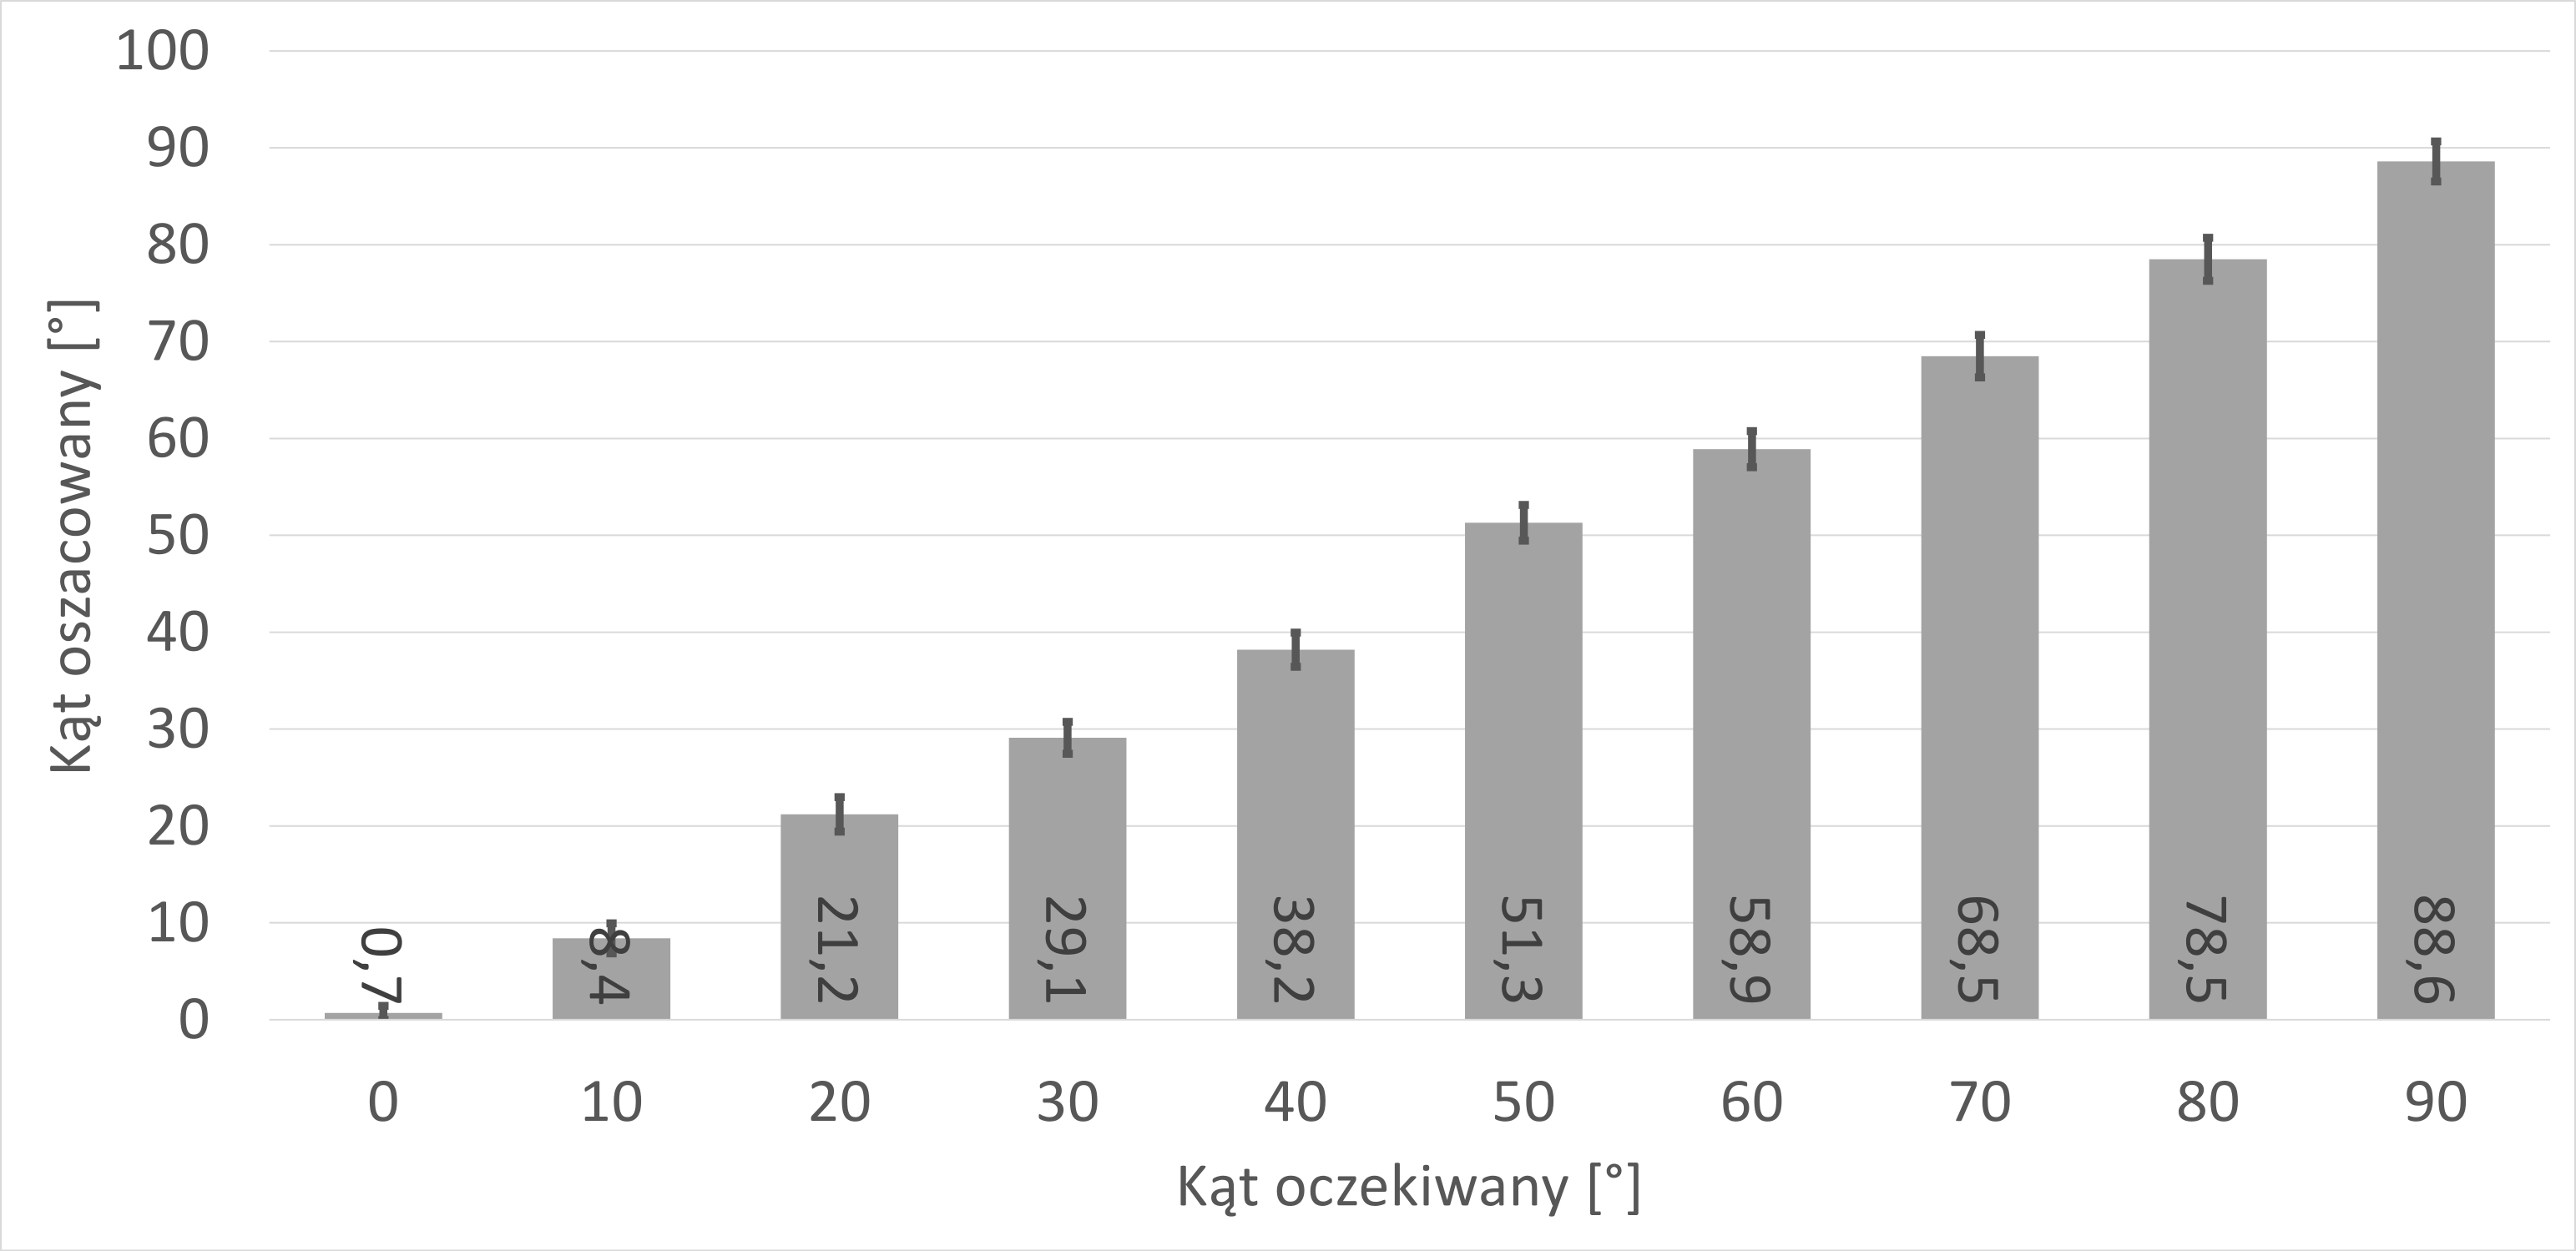
\includegraphics[width=\textwidth]{images/imumeasuredAngles.png}
		\caption{Wykres przedstawiający uśrednione wartości oszacowania kąta obrotu wokół osi $X$ i~$Y$ za pomocą modułu inercyjnego (źródło: badania własne)}
		\label{fig:hybrid:imu:XYRot}
	\end{figure}
\end{savenotes}
\begin{savenotes}
	\begin{figure}[!htb]
		\centering 
		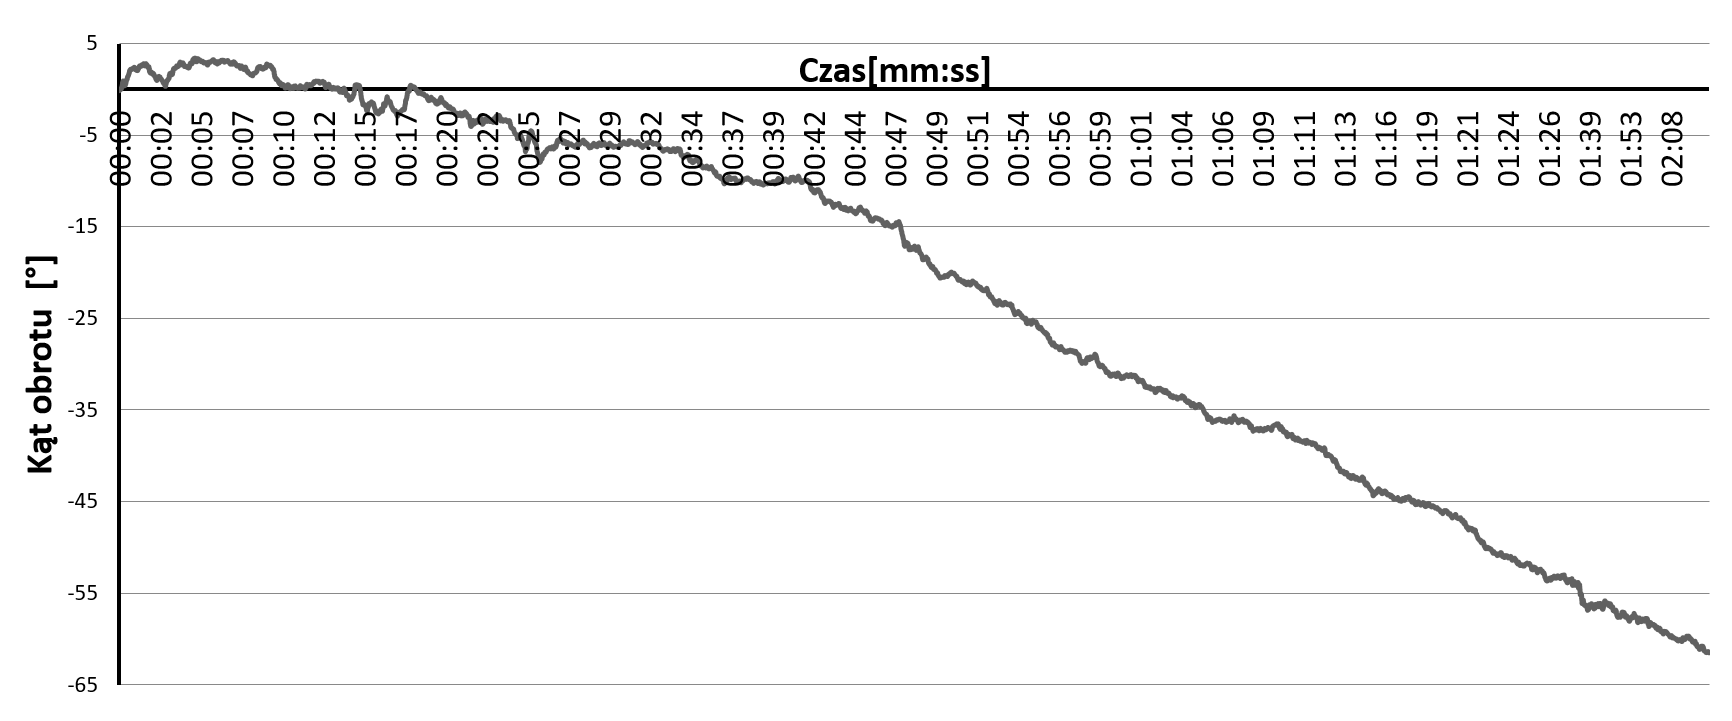
\includegraphics[width=\textwidth]{images/imuDrift.png}
		\caption{Wykres przedstawiający dryf oszacowania kąta obrotu modułu inercyjnego wokół osi $Z$ (źródło: badania własne)}
		\label{fig:hybrid:imu:drift}																														
	\end{figure}
\end{savenotes}
						
Zanim jednak dane z~akcelerometru i~żyroskopu zostaną połączone ze sobą z~wykorzystaniem filtru Madgwicka, pomiary uzyskane za pomocą akcelerometru poddane są korekcie ze względu na aktualną temperaturę pracy sensora.
\begin{equation}
	A' = \frac{A}{1+f_T (T-T_0)}
	\label{eq:hybrid:temperatureCorrection}
\end{equation}

Wzór \ref{eq:hybrid:temperatureCorrection} przedstawia sposób korekty pomiaru z~akcelerometru $A$ w~określonej temperaturze $T$. Temperatura $T_0$ to temperatura neutralna, która według specyfikacji wykorzystanego układu elektronicznego oraz na podstawie własnych badań dotyczących wpływu temperatury na dokładność pomiarów czujników inercyjnych, wynosi $25\degree C$ (wykres na rys.~\ref{fig:characteristics:imu:temp}). W~znanej mnie literaturze przedmiotu, korekta taka nie była uwzględniania lub autorzy tych publikacji nie zamieścili stosownej informacji o~tym fakcie.
						
Również dane dotyczące położenia w~przestrzeni wybranych stawów szkieletu, pobrane z~kontrolera Kinect, muszą zostać poddane filtracji. Umożliwia to zmniejszenie efektu ''drgania'' położenia stawów, których ruch jest śledzony oraz eliminuje krótkotrwałe zaburzenia śledzenia mające swój efekt w~postaci znaczących różnic w~położeniu danego stawu pomiędzy dwoma kolejnymi pomiarami. Na przykład przy częstotliwości pracy kontrolera Kinect wynoszącej 30 Hz przemieszczenie się stawu o~kilkanaście centymetrów, pomiędzy dwoma kolejnymi oszacowaniami, może wskazywać błąd wyznaczania pozycji lub błąd pomiaru. Aby ograniczyć wpływ opisanych szumów na dalsze etapy działania opracowanej przez autora hybrydowej metody śledzenia ruchu, pozycje wybranych stawów, których ruch jest śledzony, zostały poddane filtracji dolnoprzepustowej za pomocą filtru wykładniczego I-go rzędu. Jego działanie opiera się na komplementarnym łączeniu ze sobą zaszumionych danych dotyczących pozycji $P$ stawu $j$ pobranych z~kontrolera Kinect w~chwili $t$ ($P^K_{j,t}$) z~wynikiem działania filtra w~chwili $t-1$ ($P'^K_{j,t-1}$) przy zastosowaniu współczynnika filtracji $f_{LPF}$ zgodnie ze wzorem \ref{eq:hybrid:kinect:lpf}.

\begin{equation}
	\label{eq:hybrid:kinect:lpf}
	P'^K_{j,t} = f_{LPF} P^K_{j,t} + (1-f_{LPF})P'^K_{j,t-1}
\end{equation}

Przykład danych dotyczący położenia stawu łokciowego przed i~po zastosowaniu omówionego filtra wykładniczego I-go rzędu, przedstawiają wykresy z~rysunków \ref{fig:hybrid:kinect:noised} oraz \ref{fig:hybrid:kinect:denoised}.
						
	
\begin{savenotes}
	\begin{figure}[!htb]
		\centering
		\begin{subfigure}[b]{\textwidth}
			\centering
			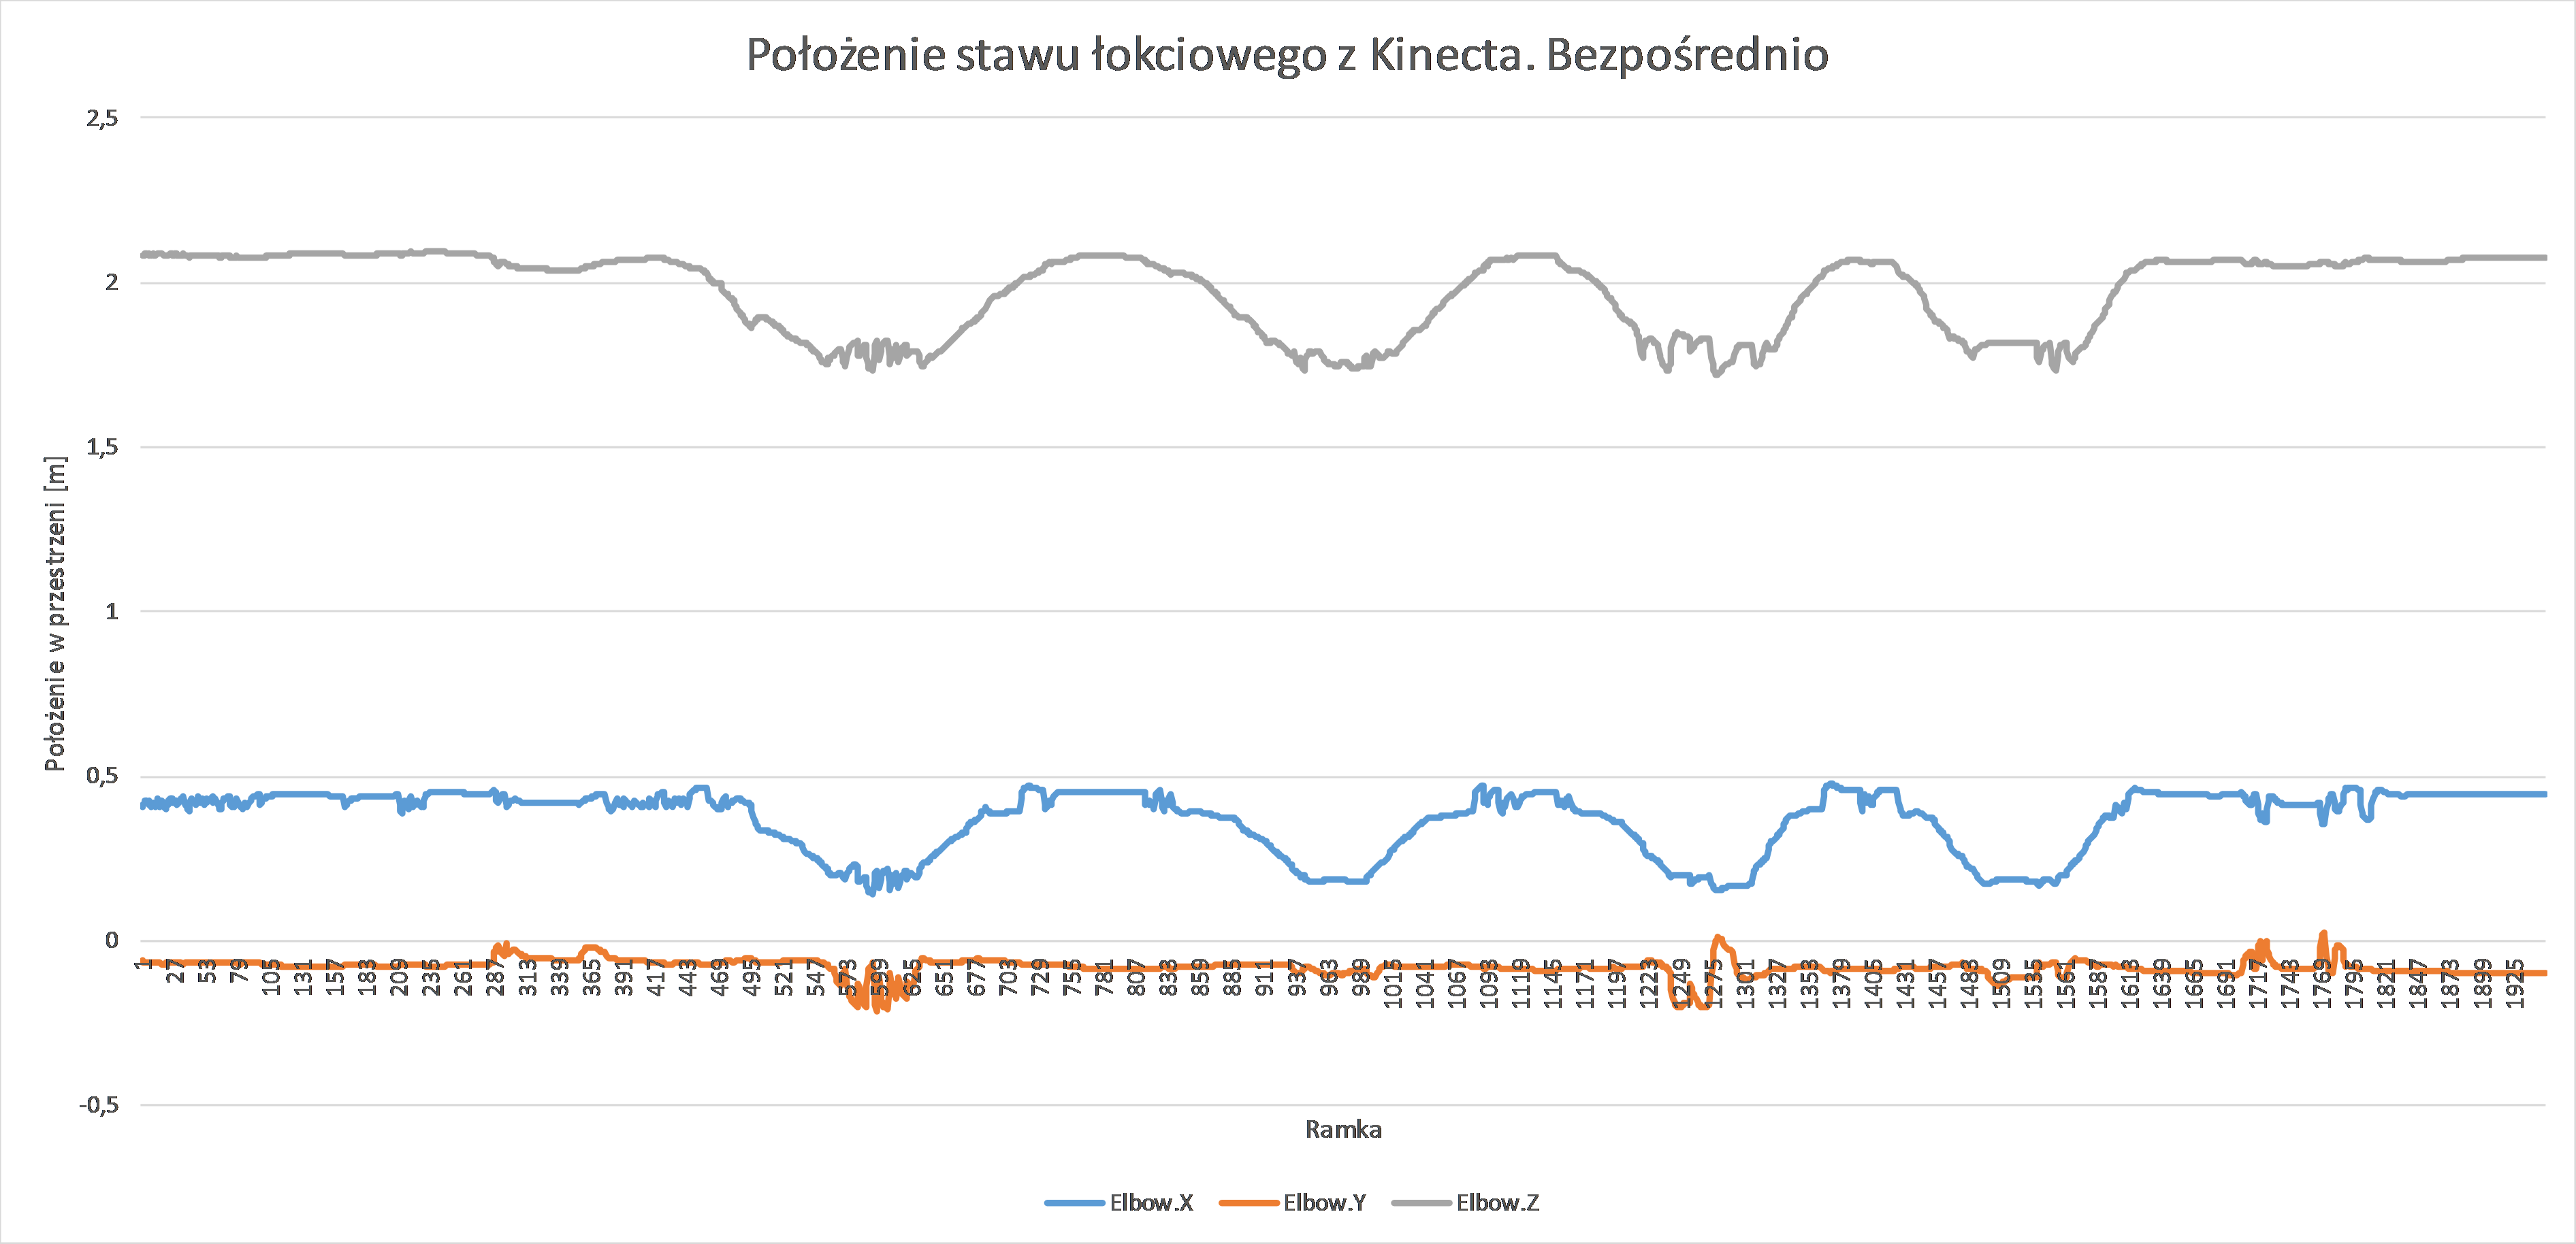
\includegraphics[width=\textwidth]{images/kinectElbowRaw.png}	
			\caption{Pomiar bezpośredni -- zaszumiony}
			\label{fig:hybrid:kinect:noised}
		\end{subfigure}
		\begin{subfigure}[b]{\textwidth}
			\centering
			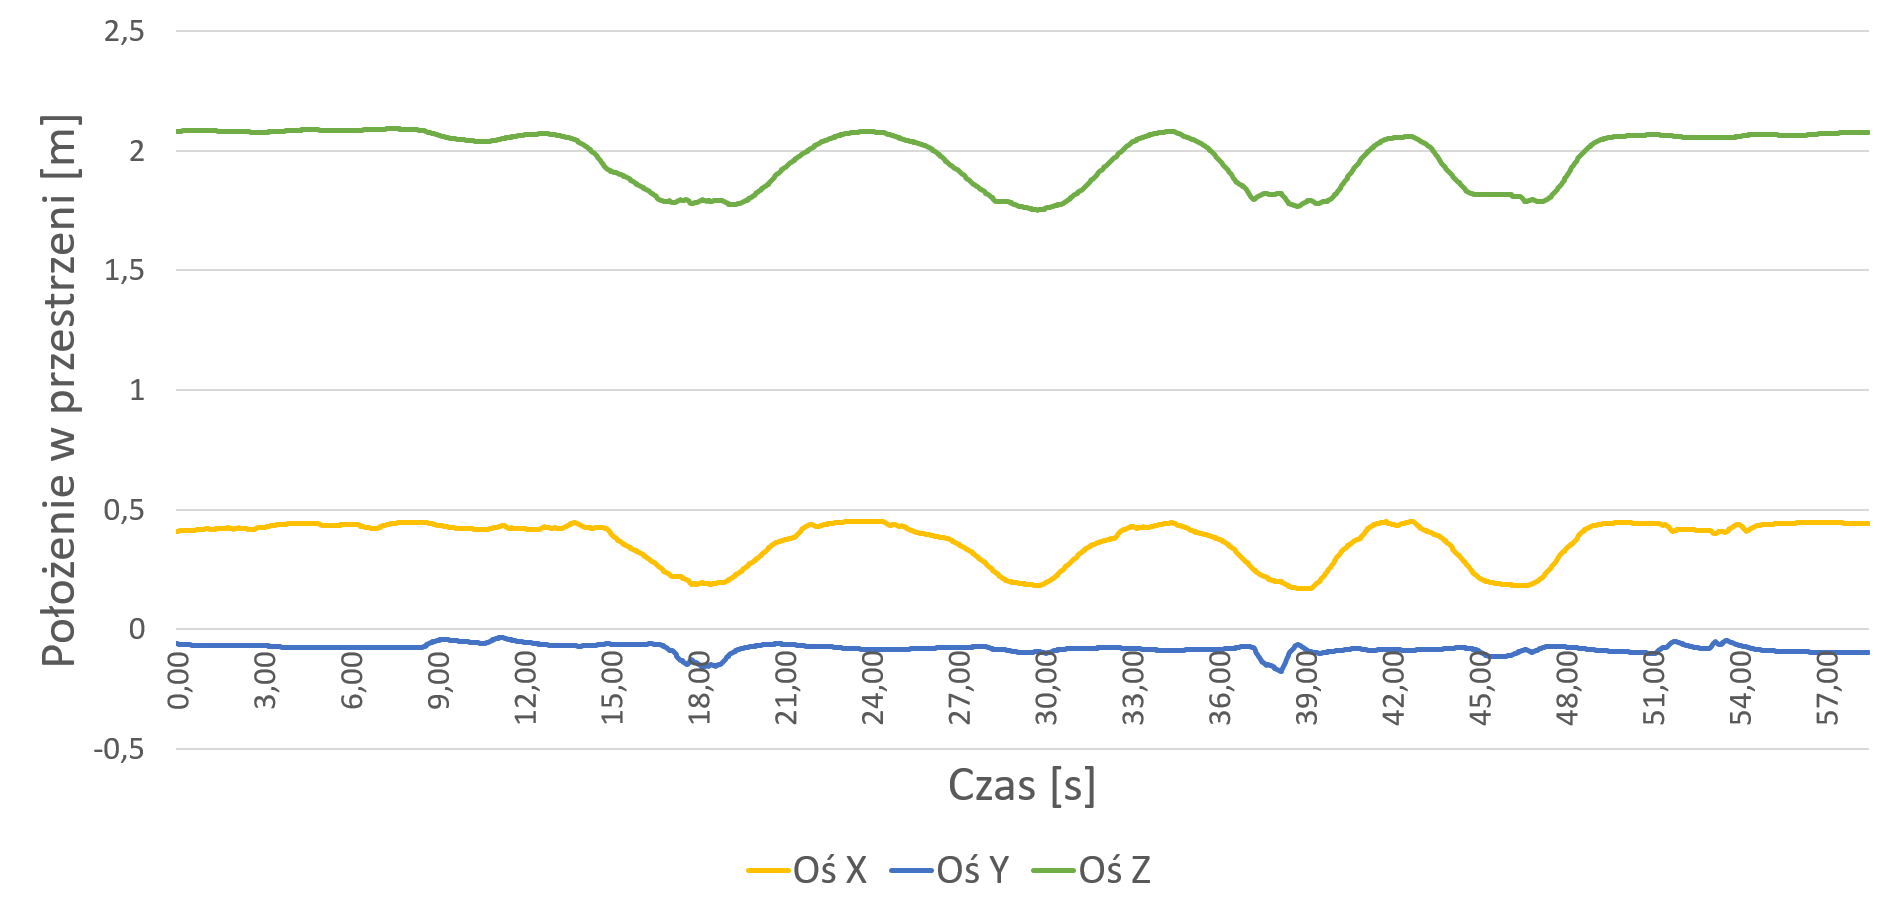
\includegraphics[width=\textwidth]{images/kinectElbowFiltered.png}	
			\caption{Pomiar odszumiony}
			\label{fig:hybrid:kinect:denoised}
		\end{subfigure}				
		\caption[Wykres przedstawiający oszacowanie położenia stawu łokciowego za pomocą kontrolera Kinect na podstawie sygnału zaszumionego oraz odszumionego]{Wykres przedstawiający oszacowanie położenia stawu łokciowego za pomocą kontrolera Kinect na podstawie sygnału zaszumionego (a) oraz odszumionego (b) filtrem wyrażonym wzorem \ref{eq:hybrid:kinect:lpf} (źródło: badania własne)}
	\end{figure}
\end{savenotes}
								
Wartość współczynnika filtracji $f_{LPF}$ została wyznaczona w~drodze prowadzonych badań własnych i~została ustalona na $0.065$. Przeprowadzone przeze mnie badanie wpływu wartości współczynnika filtracji na dokładność oszacowania pozycji stawów, za pomocą kontrolera Kinect, polegało na wyznaczeniu średniego błędu oszacowania pozycji stawów między wskazaniami kontrolera Kinect, a~danymi referencyjnymi uzyskanymi z~systemu śledzenia ruchu firmy Vicon. W~trakcie badania były wykonywane ruchy samych kończyn jak i~całego ciała, śledzone równocześnie przez system Vicon jak i~kontroler Kinect. Następnie wyznaczany był średni błąd oszacowania pozycji dla wybranych stawów, z~wykorzystaniem filtra oraz bez niego, a~także z~różnymi wartościami współczynnika $f_{LPF}$. Rysunek \ref{fig:hybrid:kinect:lpf} przedstawia wykres zależności uzyskanego średniego błędu oszacowania pozycji stawów w~zależności od wartości współczynnika filtracji $f_{LPF}$. 
								
\begin{savenotes}
	\begin{figure}[!htb]
		\centering 
		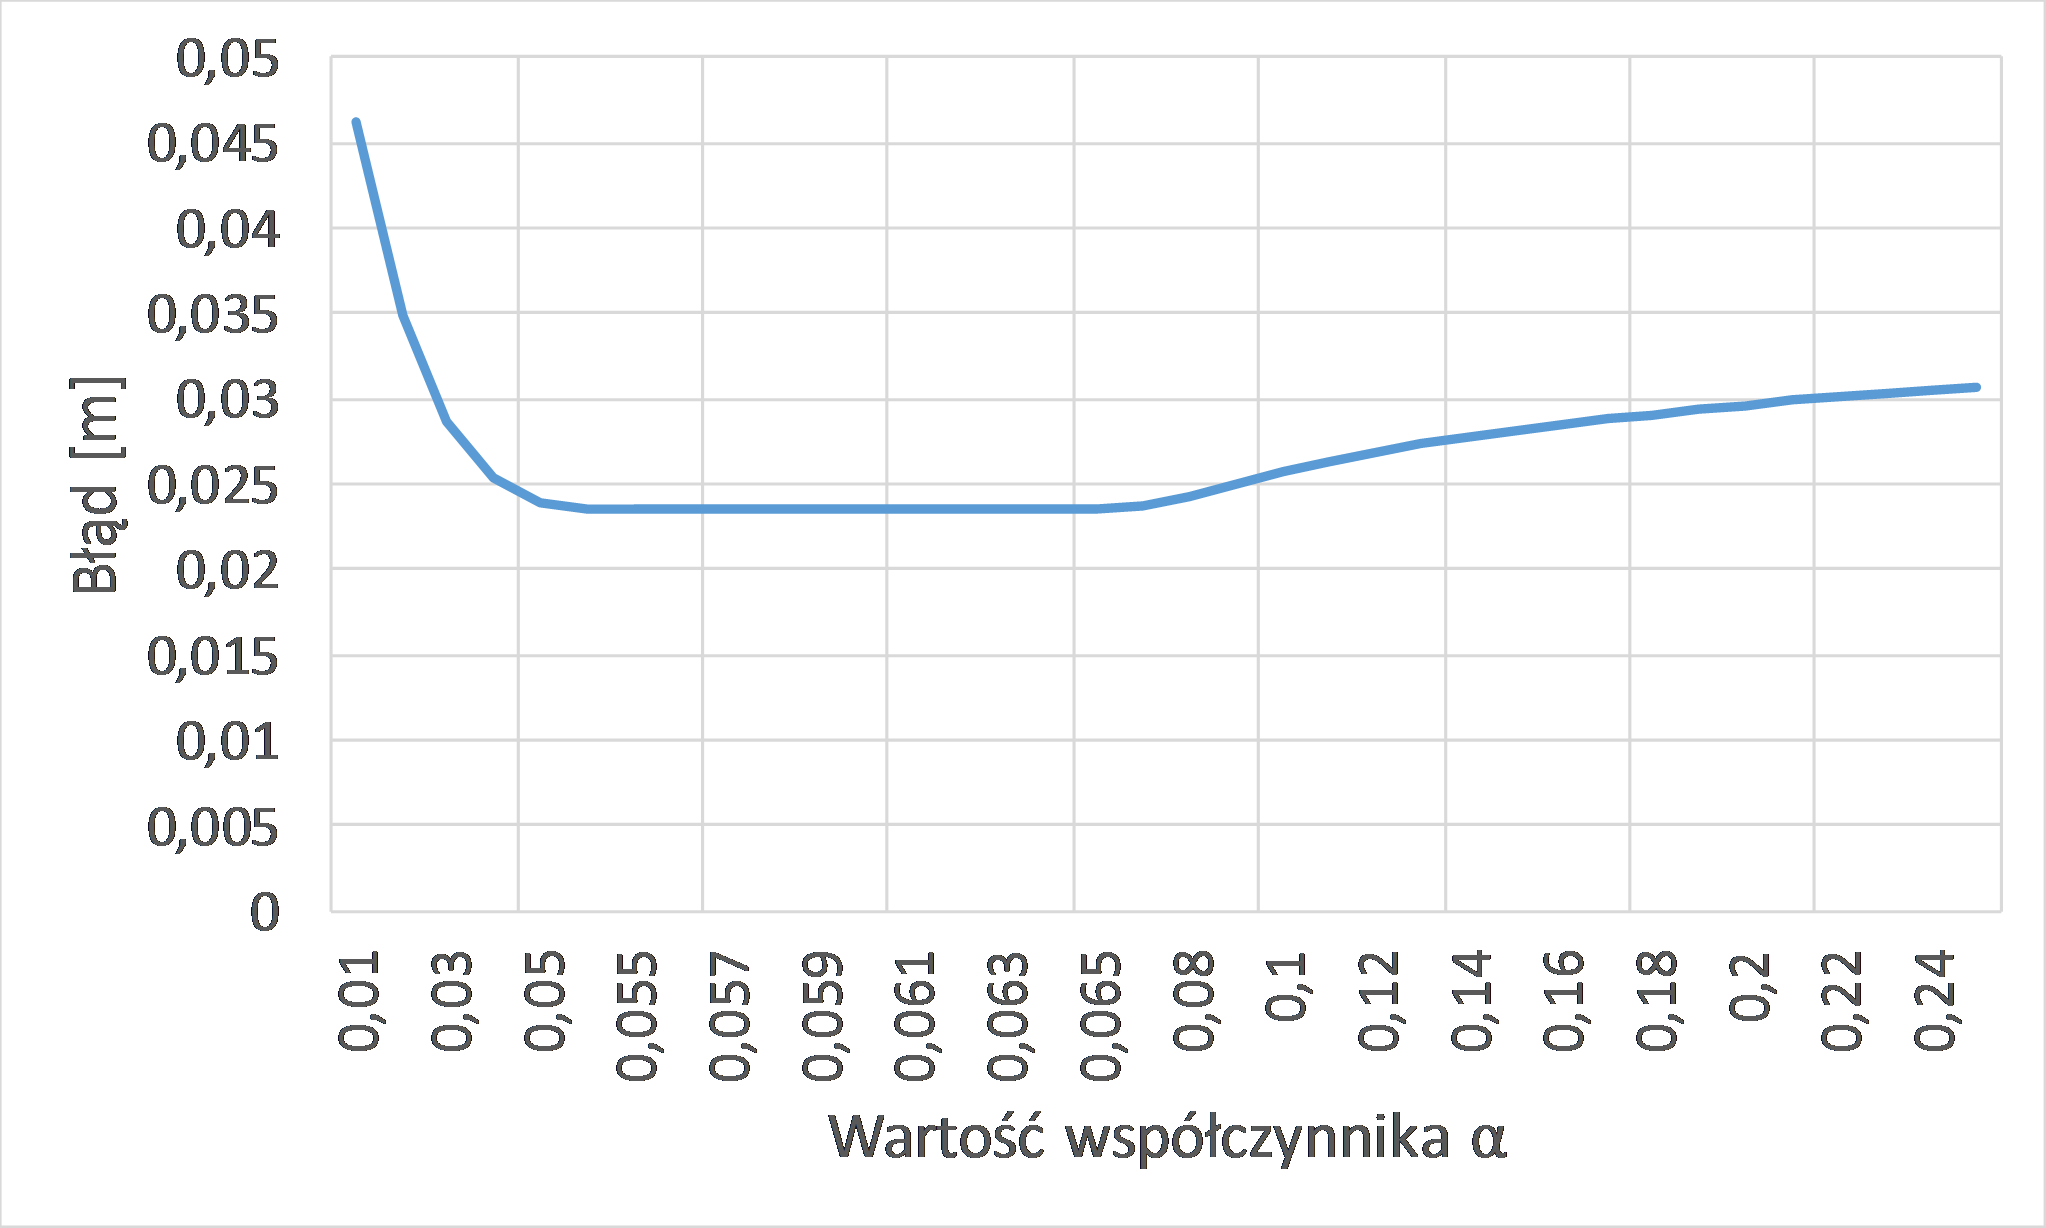
\includegraphics[width=0.75\textwidth]{images/kinectPosErrorAlpha.png}
		\caption{Wykres przedstawiający średni błąd pozycjonowania stawów za pomocą kontrolera Kinect w~zależności od współczynnika filtracji $\alpha$ (źródło: badania własne)}
		\label{fig:hybrid:kinect:lpf}
	\end{figure}
\end{savenotes}
										
Korekcie muszą zostać poddane także oszacowania odległości od kontrolera Kinect, w~jakiej znajdują się wybrane stawy. Krok ten nie był uwzględniany w~dotychczas opublikowanej, znanej autorowi literaturze, a~ze względu na zauważalną różnicę pomiędzy oszacowaniami Kinecta a~rzeczywistą odległością, w~jakiej stoi użytkownik, ma on wpływ na błędy w~dalszych obliczeniach. Zgodnie ze wzorami \ref{eq:characteristics:kinect:distanceAccuracyPoly} i~\ref{eq:characteristics:kinect:distanceAccuracyCoef}, definiującymi model błędu szacowania odległości pomiędzy osobą, której ruch jest śledzony a~Kinectem, funkcja korygująca ten błąd przybiera postać wzoru \ref{eq:distCorr}.
\begin{equation}
	f(z) = z' = -0.02z^3 + 0.11z^2 - 0.27z + 0.25
	\label{eq:distCorr}
\end{equation}

gdzie wartość $z$ to oszacowanie odległości podlegające korekcie, a~$z'$ to wartość skorygowana. Formuła korygująca oszacowanie odległości wykonane przez kontroler Kinect jest efektem własnego eksperymentu opisanego szerzej w~rozdziale \ref{sssection:distanceEstimation}.
										
\section{Synchronizacja czasowa}
										
Aby dane reprezentujące położenie badanego stawu, na podstawie czujników inercyjnych oraz kontrolera Kinect, mogły być poprawnie złączone, powinny zostać najpierw zsynchronizowane w~czasie. Jest to proces, który powinien zostać przeprowadzony przed każdą sesją śledzenia ruchu, na przykład przed konkretną sekwencją ćwiczeń do wykonania. Synchronizacja czasowa ma na celu określenie przesunięcia czasowego, jakie występuje pomiędzy oszacowaniami położenia tych samych stawów w~trakcie tego samego ruchu za pomocą każdego z~urządzeń pomiarowych osobno -- czujników inercyjnych i~kontrolera Kinect. Informacja dotycząca kroku związanego z~synchronizacją sygnałów rozważanych urządzeń nie znalazła się w~żadnej ze znanych autorowi pozycji bibliograficznych dotyczących omawianego przedmiotu, co może wskazywać na jego pominięcie w~procesie przetwarzania i~łączenia sygnałów źródłowych. To z~kolei może skutkować powstaniem błędów na skutek łączenia nie skorelowanych ze sobą danych.\\
Do wyznaczenia przesunięcia czasowego pomiędzy sygnałem uzyskiwanym z~czujników inercyjnych ($I[t]$), a~tym z~kontrolera Kinect ($K[t]$) wykorzystany został algorytm korelacji wzajemnej (\emph{ang. cross--correlation}) określony wzorem \ref{eq:cross-cor:1}.

\begin{equation}
	(I \ast K)(\tau) = \int_{-\infty}^{+\infty}I[t]K[t+\tau]dt
	\label{eq:cross-cor:1}
\end{equation}

Parametr $\tau$ odpowiada za opóźnienie jednego sygnału względem drugiego. Aby wyznaczyć jakie jest przesunięcie czasowe ($\tau_{max}$) pomiędzy dwoma sygnałami należy znaleźć taką wartość argumentu $\tau$ dla której wartość funkcji korelacji wzajemnej pomiędzy badanymi sygnałami jest największa, co przedstawia wzór \ref{eq:cross-cor:2}.										
										
\begin{equation}
	\tau_{max}       = \underset{\tau}{argmax}((I \ast K)(\tau))
	\label{eq:cross-cor:2} 
\end{equation}

Aby można było skutecznie wyznaczyć tę wartość, oba sygnały muszą posiadać tę samą częstotliwość próbkowania. Spełnienie tego warunku uzyskano poprzez obniżenie częstotliwości próbkowania sygnału uzyskanego z~czujników inercyjnych ze 100Hz  do 30Hz, to znaczy została ona zrównana do tej, z~jaką pracuje Kinect. Pomiary z~czujników inercyjnych są tymczasowo buforowane i~gdy zostanie pobrany pakiet danych z~Kinecta, pomiary z~modułów inercyjnych zgromadzone w~tymczasowym buforze zostają poddane filtrowi medianowemu, aby wyeliminować ewentualne krótkotrwałe zaburzenia pomiarów. 
										
W~znanej autorowi niniejszej dysertacji literaturze przedmiotu, korekta taka nie była uwzględniania lub autorzy tych publikacji nie zamieścili stosownej informacji o~tym fakcie.

Wyznaczona wartość przesunięcia w~czasie pomiędzy sygnałami ($\tau_{max}$) wykorzystywana jest następnie do modyfikacji wartości znacznika określającego czas odebrania danych z~modułu inercyjnego przez komputer PC. Tak zmodyfikowany znacznik czasu wykorzystywany jest do wyznaczenia pomiarów z~czujników inercyjnych odpowiadających pomiarom uzyskanym z~kontrolera Kinect. Metoda określająca odpowiadające sobie pomiary z~kilku sygnałów, na podstawie czasów otrzymania wartości każdego z~badanych sygnałów, nazywana jest decymacją \cite{Hinton2001}. Przyjmując, że $t_K$ jest znacznikiem czasowym otrzymania na komputerze PC danych z~kontrolera Kinect, a~$t_I[]$ to zbiór znaczników czasowych próbek otrzymanych z~czujników inercyjnych i~umieszczonych w~buforze, wówczas wybór próbki danych pomiarowych z~czujników inercyjnych skorelowanych z~danymi z~kontrolera Kinect wyrażony jest wzorem \ref{eq:dec}
										
\begin{equation}
	i_{res} = \underset{i}{argmin}(|t_K-(t_I[i] + \tau_{max})|)
	\label{eq:dec}
\end{equation}

gdzie $i_{res}$ to numer próbki umieszczonej w~buforze danych odpowiadającej danym otrzymanym z~Kinecta ze znacznikiem czasowym $t_K$.
										
W trakcie prowadzonych autorskich prac badawczych, oprócz wyznaczenia przesunięcia czasowego pomiędzy czujnikami inercyjnymi, a~kontrolerem Kinect, zostało zbadane przesunięcie czasowe pomiędzy tymi urządzeniami pomiarowymi, a~systemem śledzenia ruchu Vicon. Przyjmując, że Vicon działa w~czasie rzeczywistym, przesunięcia te określają de facto jakie jest opóźnienie między IMU i~Kinectem, a~rzeczywistym ruchem. I~tak, średnie przesunięcie czasowe pomiędzy czujnikami inercyjnymi a~systemem Vicon wyniosło około $0.04s$, natomiast pomiędzy Kinectem a~systemem Vicon to około $0.09s$. Korelacja wyznaczona między czujnikami inercyjnymi a~kontrolerem Kinect wskazuje, że średnie przesunięcie szacowania pozycji wynosi około $0.06s$. Z~uwagi na to, że dane z~czujników inercyjnych są łączone z~pomiarami uzyskanymi z~kontrolera Kinect, zgodnie z~częstotliwością pracy Kinecta, zasadnym jest wskazanie, że opisywana przez autora metoda łączenia danych ze wspomnianych urządzeń posiada opóźnienie $0.09s$ względem rzeczywistego ruchu.
										
\section{Łączenie danych}
										
Strumienie danych pochodzące z~poszczególnych sensorów, zsynchronizowane czasowo oraz poddane filtracji mogą zostać połączone celem uzyskania wypadkowych wartości, lepiej odzwierciedlających układ szkieletu śledzonej postaci. Na tym etapie prezentowana metoda opiera się na informacji o~orientacji przestrzennej poszczególnych kości zamiast na położeniu konkretnych stawów. Jest to nowe podejście do łączenia sygnałów z~czujników inercyjnych z~sygnałami z~kontrolera Kinect, które stanowi jedno z~głównych osiągnięć prezentowanej pracy. Podejście takie podyktowane jest faktem, że w~przypadku czujników inercyjnych, wyznaczenie położenia stawów wymaga połączenia informacji o~orientacji przestrzennej czujników z~modelem szkieletowym zawierającym informację o~długościach poszczególnych kości. Z~uwagi, że wykorzystując definicję modelu szkieletowego, definicja długości jego segmentów jest stała, należy zwrócić szczgólną uwagę na dokładność pomiarów tych długości. Wszelkie błędy i~niedokładności popełnione na tym etapie przygotowywania modelu mogą skutkować pojawieniem się istotnych błędów w~oszacowaniu położenia poszczególnych stawów. Co więcej, ze względu na hierarchiczną budowę modelu szkieletowego, ewentualne błędy wynikające z~braku dokładnych pomiarów długości poszczególnych kości szkieletu będą się kumulowały wraz z~odległością danego segmentu od korzenia. 

Wykorzystanie położenia stawów szkieletu, w~procesie łączenia sygnałów z~obu źródeł, dodatkowo utrudnia fakt niedokładności w~oszacowaniu modelu szkieletowego za pomocą kontrolera Kinect. Model ten nie ma zdefiniowanych długości poszczególnych kości na stałe (choćby na czas pojedynczej sesji śledzenia) i~są one determinowane przez oszacowanie położenia kolejnych stawów, obarczonych zauważalną zmiennością w~czasie. To z~kolei skutkuje tym, że długości poszczególnych kości modelu szkieletowego, oszacowanego przez kontroler Kinect, różnią się nawet o~kilka $cm$ pomiędzy kolejnymi pomiarami.
										
Dane z~obu źródeł (kontroler Kinect i~moduł inercyjny) zawierają informacje o~orientacji przestrzennej wyrażone w~kwaternionach, jednak dalsze obliczenia, mające na celu połączenie tych informacji, są bardziej intuicyjne przy reprezentacji w~postaci kątów Eulera. Konwersja taka przeprowadzona jest zgodnie ze wzorem \ref{eq:appx:rot:quatToEuler}, a~w~jej wyniku wartości obrotów wokół każdej z~osi układu współrzędnych danego urządzenia pomiarowego, które składają się na orientację przestrzenną danej kości, są wyrażone bezpośrednio. Reprezentacja w~postaci kątów Eulera ułatwia także konwersję informacji o~obrotach do wspólnego, globalnego układu współrzędnych, co jest niezbędne, żeby można było je w~dalszych krokach łączyć. Informacje o~orientacji kości, wyznaczone na podstawie danych pomiarowych z~czujników inercyjnych oraz kontrolera Kinect, są od siebie niezależne i~uzupełniają się nawzajem. Wzajemna niezależność i~uzupełnianie się danych umożliwia ich połączenie w~sposób komplementarny. Łącząc dane w~sposób komplementarny, każdej z~wartości podlegającej łączeniu przypisane zostają wagi, których suma wynosi $1$, a~następnie są one ze sobą sumowane z~uwzględnieniem wag określających poziom istotności poszczególnych wartości kątów. Wynik sumowania reprezentuje wartość złączonych danych wejściowych. \\
										
Prezentowana w~niniejszej dysertacji hybrydowa metoda śledzenia ruchu kończyn człowieka łączy ze sobą dane pochodzące z~dwóch źródeł. Dane te są w~postaci trójelementowych wektorów orientacji $E^i = \begin{bmatrix} \phi &  \theta & \psi \end{bmatrix}^i$ ($i = \{I,K\}, I-\text{IMU}; K-\text{Kinect}$), gdzie każdy z~elementów oznacza obrót wokół pojedynczej osi układu współrzędnych -- odpowiednio $X \quad Y \quad Z$. Wektor ten stanowi reprezentację orientacji przestrzennej segmentu szkieletu w~postaci kątów Eulera, wyznaczoną przez konwersję kwaternionów otrzymanych na podstawie pomiarów czujników inercyjnych ($E^I$) lub~kontrolera Kinect($E^K$). Wagi wykorzystywane w~procesie łączenia danych są wyznaczane indywidualnie dla każdego z~elementów wektora. Przyjmując, że wagi $w_\phi , w_\theta , w_\psi$ oznaczają poziom istotności informacji otrzymanych na podstawie pomiarów czujników inercyjnych ($E^I = \begin{bmatrix}  \phi^I &  \theta^I &  \psi^I \end{bmatrix}$), wówczas komplementarne łączenie ich z~danymi otrzymanymi z~kontrolera Kinect ($E^K = \begin{bmatrix}  \phi^K &  \theta^K &  \psi^K \end{bmatrix}$) dla danej chwili $t$ pozwala oszacować złączone kąty Eulera $E^F$ ($F$ -- złączone, \emph{ang. Fused}) według wzoru \ref{eq:hybrid:reliableFusion}
										
\begin{equation} E^F_t = 
	\begin{bmatrix}  \phi^F \\  \theta^F \\  \psi^F \end{bmatrix}_t = 
	\begin{bmatrix} w_\phi * \phi^I \\ w_\theta * \theta^I \\ w_\psi * \psi^I \end{bmatrix}_t + 
	\begin{bmatrix} (1-w_\phi) * \phi^K \\ (1-w_\theta) * \theta^K \\ (1-w_\psi) * \psi^K \end{bmatrix}_t
	\label{eq:hybrid:reliableFusion}
\end{equation}
										
Wzór \ref{eq:hybrid:reliableFusion} jest wykorzystywany zawsze wtedy, kiedy dane podlegające łączeniu są dobrej jakości i~możemy je uznać za prawidłowe. W~takiej sytuacji współczynniki wag $w_\phi , w_\theta , w_\psi$ są wartościami stałymi dobranymi eksperymentalnie przez autora i~wynoszącymi odpowiednio $0.98,0.05,0.65$.\\
Waga $w_\phi$ odpowiada za obrót wokół osi przechodzącej wzdłuż ciała (oś $X$, rys.~\ref{fig:characteristics:kinect:space} i~\ref{fig:handAxes}). Wysoka wartość tej wagi wynika z~faktu, że wartość obrotu wokół tej osi jest mierzalna jedynie przez czujniki inercyjne. Dzięki wadze zbliżonej do wartości $1$, pomiary uzyskane z~Kinecta są niemal ignorowane.\\
$w_\theta$ jest wagą określającą istotność informacji o~obrocie wokół osi zgodnej z~kierunkiem działania grawitacji (oś $Y$, rys.~\ref{fig:characteristics:kinect:space} i~\ref{fig:handAxes}). Wartość tego obrotu jest bardziej wiarygodnie i~stabilnie szacowana w~czasie przez kontroler Kinect. Niska wartość wagi $w_\theta$ zmniejsza wpływ danych wyznaczonych na podstawie pomiarów czujników inercyjnych (obarczonych znaczącym dryfem) na wartości wypadkowe będące wynikiem łączenia danych.\\ 
Waga $w_\psi$ określa poziom istotności informacji o~obrocie wokół osi skierowanej w~stronę obserwacji kontrolera Kinect (rys.~\ref{fig:characteristics:kinect:space}). Obrót ten jest szacowany zarówno przez kontroler Kinect jak i~na podstawie pomiarów z~czujników inercyjnych. Oszacowania te mają jednak różną dokładność i~różnica ta jest odzwierciedlona w~przyjętej empirycznie wartości wagi. Według badań opublikowanych przez twórcę filtru Madgwicka \cite{Madgwick2010}, wykorzystywanego w~niniejszej pracy, jego metoda wyznaczania orientacji przestrzennej, na podstawie pomiarów z~czujników inercyjnych, zapewnia dokładność około $\pm2\degree$. W~badaniach własnych autora dokładność ta była zbliżona do $\pm3\degree$. Z~kolei dokładność oszacowania obrotu wokół osi $Z$ kontrolera Kinect (rys.~\ref{fig:characteristics:kinect:space}, rys.~\ref{fig:handAxes}) przez to właśnie urządzenie, określona na podstawie badań własnych jak i~opisów dostępnych w~literaturze \cite{Huber2015}, wynosi około $\pm6\degree$. Niemal dwukrotnie mniejszy błąd oszacowania obrotu wokół osi $Z$, na podstawie pomiarów z~czujników inercyjnych, ma swoje przełożenie na wartość wagi $w_\psi$.\\
Rysunek \ref{fig:handAxes} przedstawia układ współrzędnych wraz z~obrotami odpowiadającymi każdej z~osi tego układu, w~odniesieniu do ręki człowieka.
										
\begin{savenotes}
	\begin{figure}[!htb]
		\centering	
		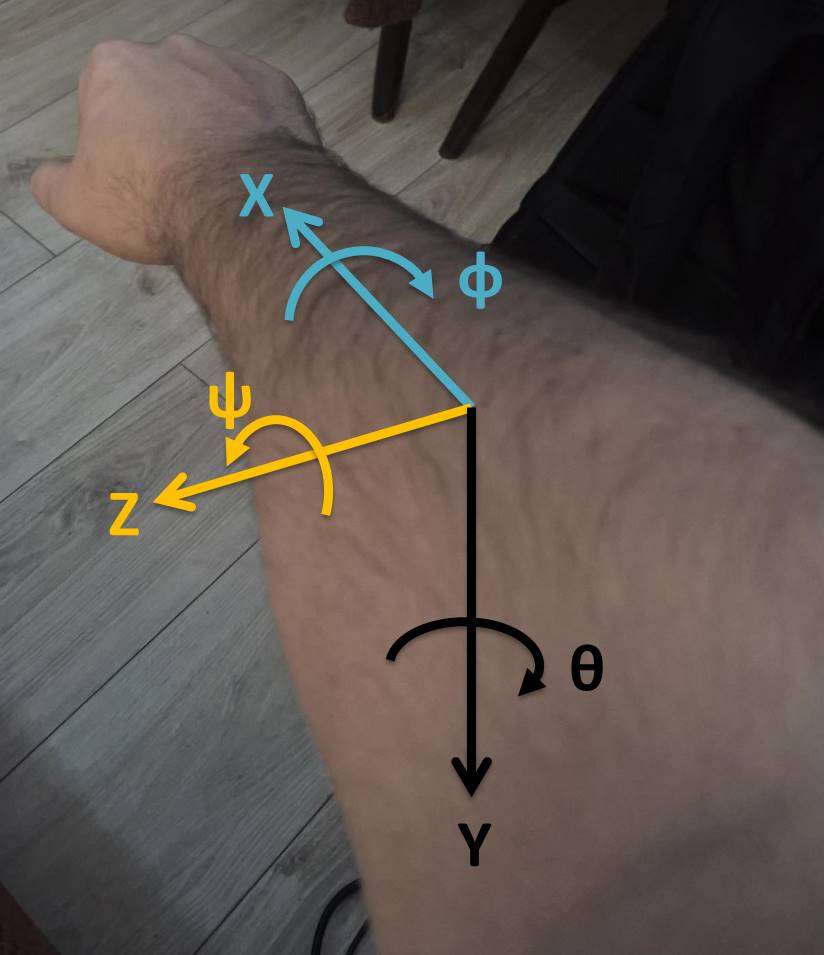
\includegraphics[width=0.6\textwidth]{images/handAxes.jpg}	
		\caption{Oznaczenie układu współrzędnych $XYZ$ wraz z~obrotami $\phi , \theta , \psi$ w~odniesieniu do ręki człowieka (źródło: opracowanie własne)}
		\label{fig:handAxes}
	\end{figure}
\end{savenotes}
												
Określenie czy oszacowania kątów, uzyskane za pomocą kontrolera Kinect, są wystarczającej jakości do łączenia ich z~oszacowaniami kątów uzyskanymi z~czujników inercyjnych, wykonywane jest każdorazowo na podstawie kryteriów związanych z~realizowanym ruchem. \\
Pierwszym kryterium branym pod uwagę jest obrót całej sylwetki względem kamery, liczony jako kąt $\alpha$ pomiędzy linią barków a~kamerą w~płaszczyźnie $X$--$Z$ (rys.~\ref{fig:characteristics:kinect:bodyRotationAngle}) zgodnie ze wzorem \ref{eq:characteristics:kinect:bodyRotationAngle}. Na podstawie zbadanych wcześniej charakterystyk obu urządzeń wiadomo, że dane które można wiarygodnie wykorzystać do łączenia są możliwe do uzyskania tylko gdy sylwetka nie jest obrócona o~więcej niż $50\degree$. Oprócz wartości kąta obrotu sylwetki brane jest także pod uwagę odchylenie standardowe estymacji tego obrotu. Przyjmując, że $\alpha[]$ to zbiór wartości oszacowań kąta obrotu sylwetki z~ostatnich $3s$ (ok. 90 elementów w~zbiorze), a~$\overline{\alpha}$ to średnia arytmetyczna elementów w~tym zbiorze, wówczas odchylenie standardowe $\sigma_\alpha$ definiuje wzór \ref{eq:stdDev}.
												
\begin{equation}
	\sigma_\alpha = \sqrt{\frac{1}{n}\sum_{i=1}^{n}{(\alpha[i] - \overline{\alpha})^2}}
	\label{eq:stdDev}
\end{equation}
												
Branie pod uwagę zarówno wartości estymacji obrotu sylwetki wraz z~odchyleniem standardowym uzyskiwanych oszacowań spowodowane jest faktem, że w~momencie wystąpienia okluzji jednego lub obu stawów barkowych i~błędów oszacowania ich położenia, następuje błędne oszacowanie wartości obrotu. W~praktyce oznacza to, że wyznaczony kąt obrotu sylwetki może przyjąć dowolną wartość. Przykład szacowania kąta obrotu sylwetki względem kontrolera Kinect przedstawia wykres z~rysunku \ref{fig:hybrid:kinect:kinectRotationVariance}. W~trakcie tego eksperymentu badawczego wykonywany był obrót postaci względem kontrolera Kinect do kąta $90\degree$ i~powrót do pozycji równoległej do urządzenia pomiarowego, czyli do kąta $0\degree$. Przy obrocie sylwetki nie przekraczającym $50\degree$ odchylenie standardowe oszacowań z~przyjętego okresu czasu nie przekraczało wartości $1.5\degree$. W~związku z~tym w~opisywanej w~niniejszej dysertacji hybrydowej metodzie śledzenia ruchu kończyn człowieka, autor przyjął, że pomiar obrotu postaci w~stosunku do kontrolera Kinect jest wiarygodny, jeśli oszacowanie jego kąta obrotu jest $\alpha \le 50\degree$ przy odchyleniu standardowym $\sigma_\alpha\le 1.5 \degree$.
												
\begin{savenotes}
	\begin{figure}[!htb]
		\centering
		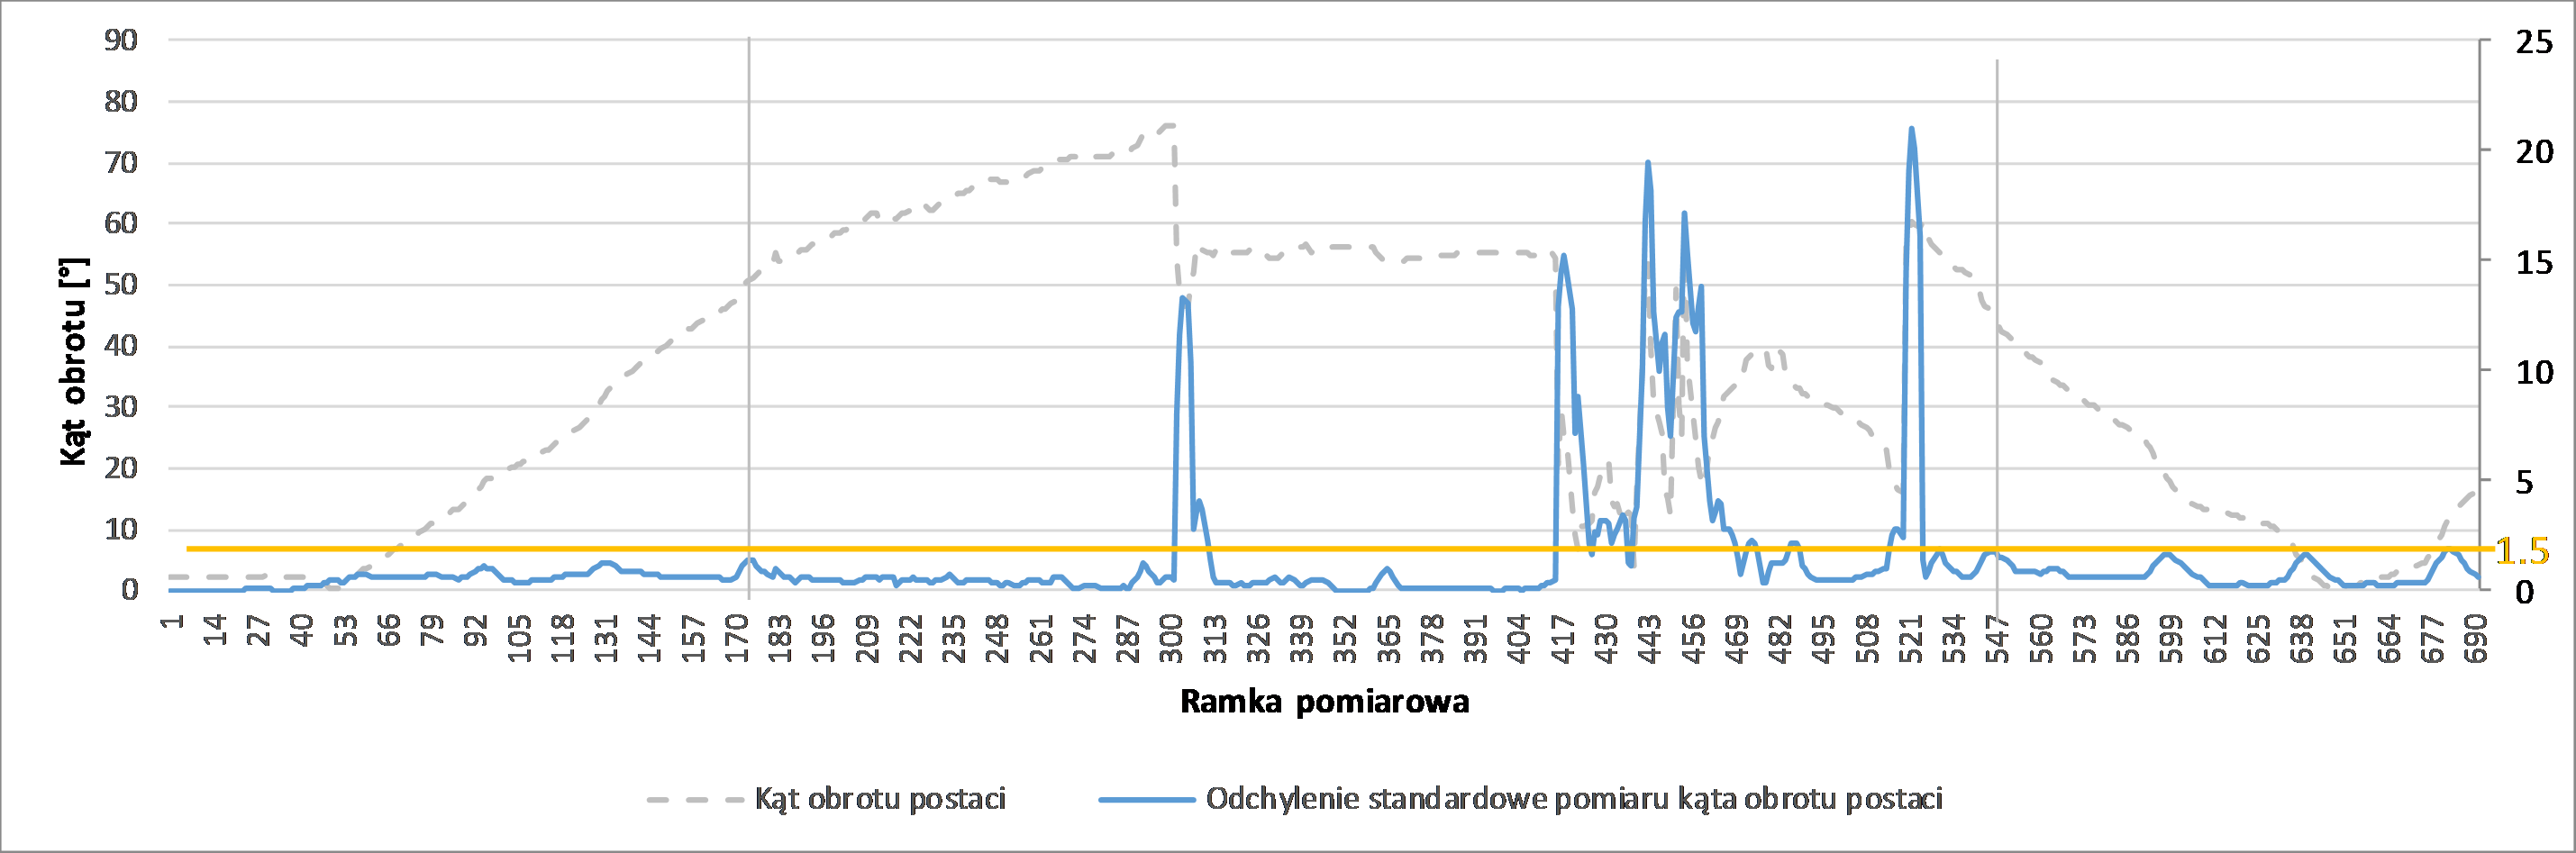
\includegraphics[width=\textwidth]{images/kinectRotationStdDev.png}
		\caption{Odchylenie standardowe estymacji kąta obrotu postaci względem Kinecta  (źródło: badania własne)}						
		\label{fig:hybrid:kinect:kinectRotationVariance}
	\end{figure}
\end{savenotes}
														
Oprócz obrotu całej postaci, ocenie podlega także stabilność pomiarów samych stawów. Pierwszym parametrem, jaki brany jest pod uwagę, jest stan śledzenia poszczególnych stawów, który może przyjąć jedną z~trzech wartości opisanych szerzej w~podrozdziale \ref{ssec:characteristics:kinect:limitation}. Wartość \emph{NotTracked} jest od razu traktowana jako wskazanie, że dane związane z~danym stawem (jego pozycja, ale także orientacja kości z~nim związanych) są niewiarygodne. W~przypadku pozostałych dwóch możliwych stanów śledzenia stawu, sprawdzany jest poziom szumu za pomocą filtru górnoprzepustowego w~postaci wzoru \ref{eq:hybrid:kinect:hpf}. 
														
\begin{equation}
	n^K_{j,t} = f_{HPF} * (n^K_{j,t-1} + P^K_{j,t} - P^K_{j,t-1}) 
	\label{eq:hybrid:kinect:hpf}
\end{equation}
														
gdzie: $n^K_{j,t}$ to poziom szumu $n$ w~aktualnym oszacowaniu położenia danego stawu $j$ w~czasie $t$ dla Kinecta, $n^K_{j,t-1}$ -- poziom szumu $n$ w~poprzednim oszacowaniu położenia danego stawu $j$ w~czasie $t-1$ dla Kinecta,	$P^K_{j,t}$ jest położeniem $P$ stawu $j$ w~aktualnym oszacowaniu $t$ dla Kinecta, $P^K_{j,t-1}$ to położenie  $P$ stawu $j$ w~poprzednim oszacowaniu $t-1$ dla Kinecta, natomiast $f_{HPF}$ jest współczynnikiem filtracji  $f_{HPF} = 0.01$. 
												
\begin{savenotes}
	\begin{figure}[!htb]
		\centering 
		\begin{subfigure}[b]{\textwidth}
			\centering
			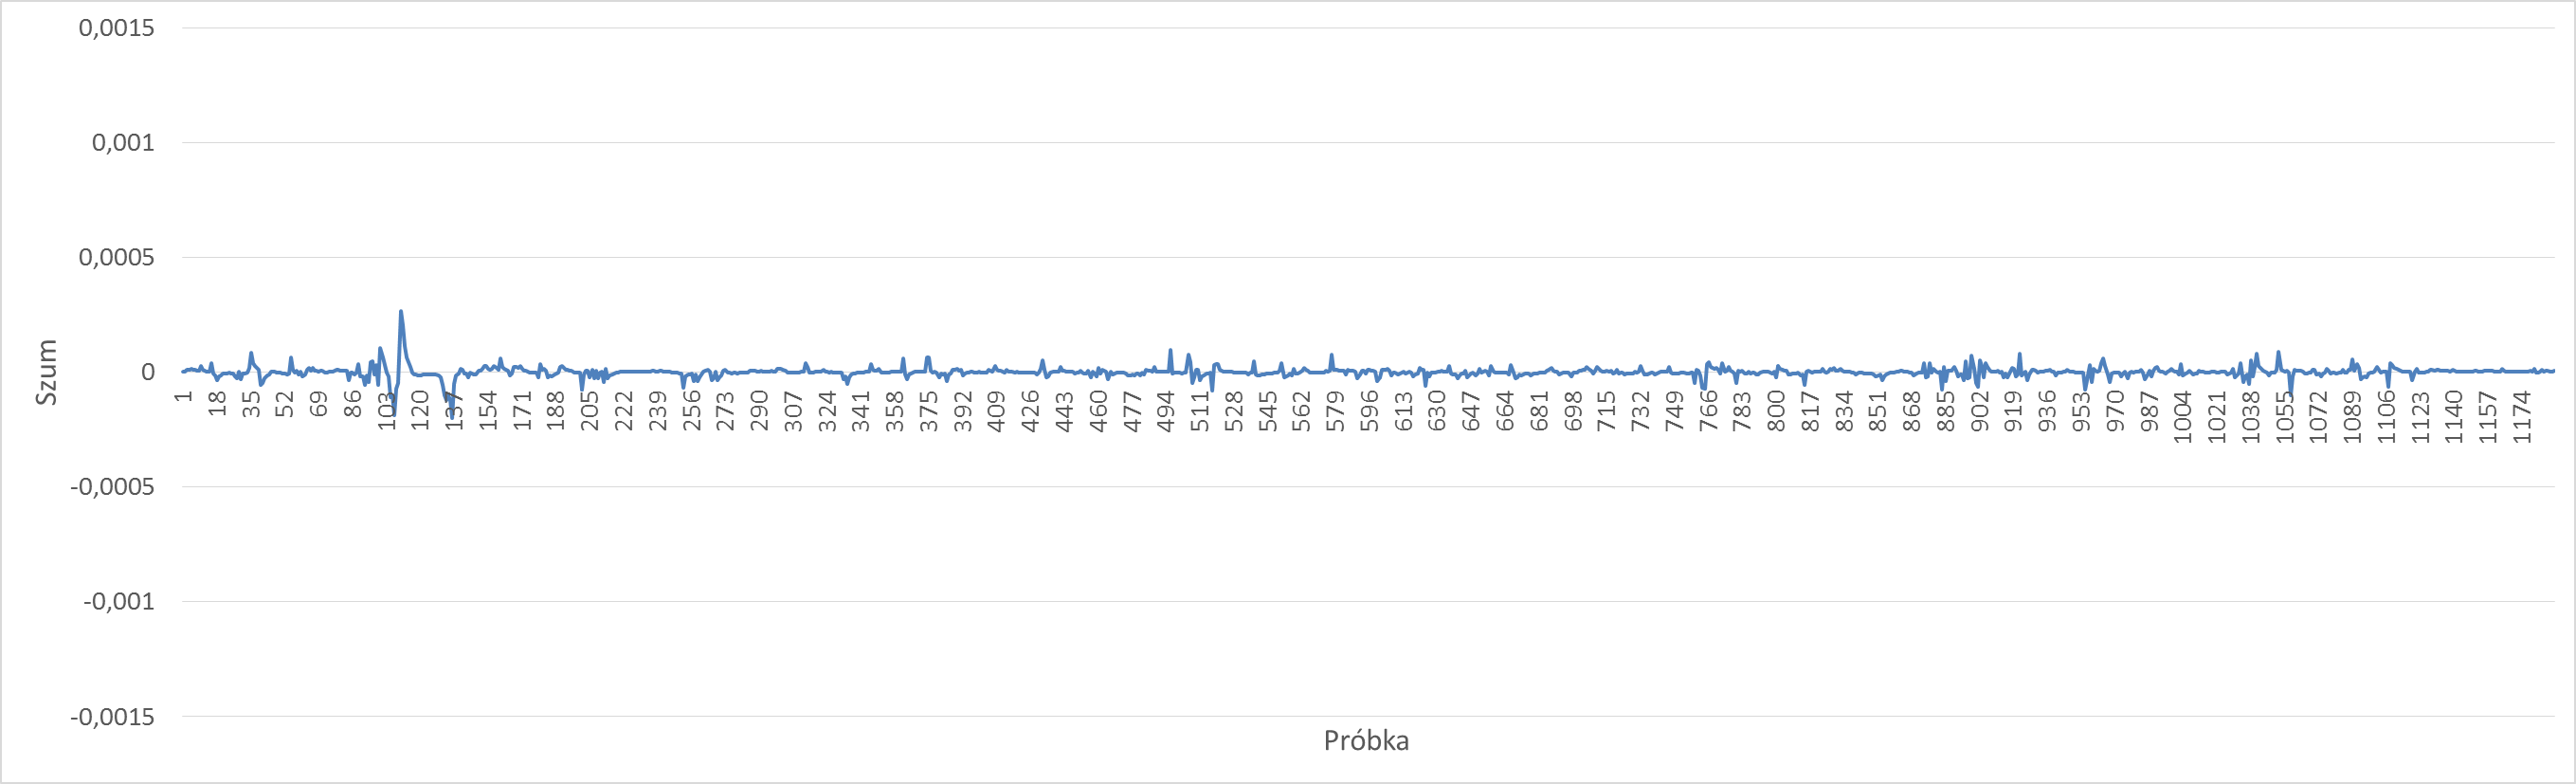
\includegraphics[width=\textwidth]{images/Fig09.png}	
			\caption{Staw śledzony ze statusem \emph{Tracked}}
			\label{fig:hybrid:kinect:hpfNotOccluded}
		\end{subfigure}	
																																									
		\begin{subfigure}[b]{\textwidth}
			\centering
			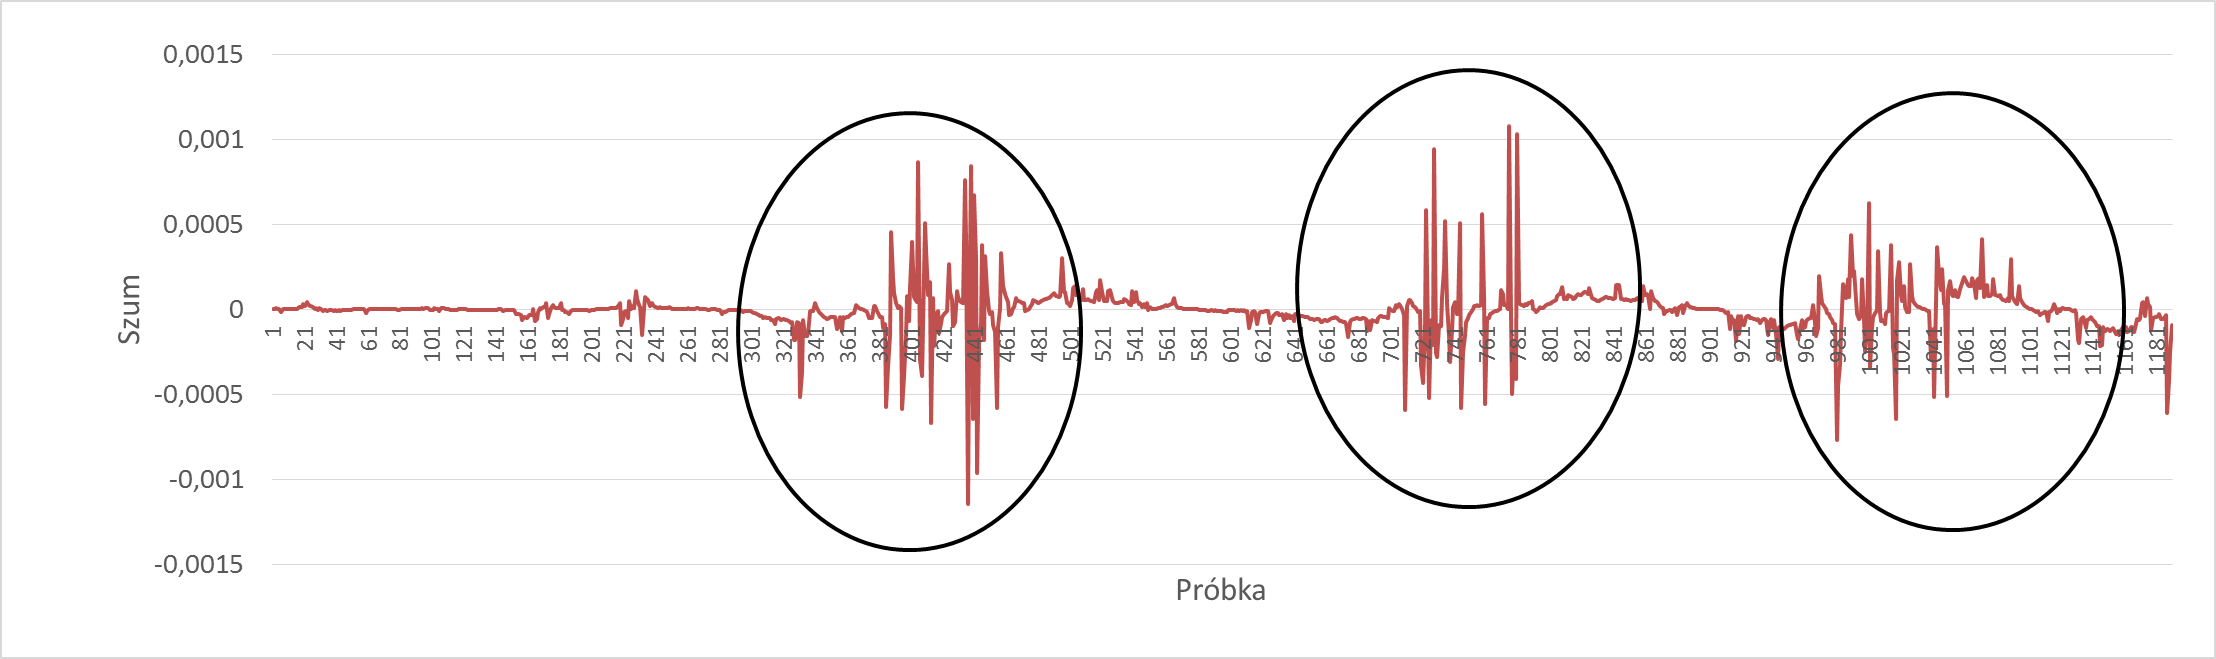
\includegraphics[width=\textwidth]{images/Fig10.png}
			\caption[Staw śledzony ze statusami \emph{Tracked} i~\emph{Interferred}]{Staw śledzony ze statusami \emph{Tracked} i~\emph{Interferred} (oznaczone owalem)}
			\label{fig:hybrid:kinect:hpfOccluded}
		\end{subfigure}	
		\caption[Wykres wartości szumu w~oszacowaniach kontrolera Kinect]{Wykres wartości szumu występującego w~oszacowaniach do położenia wybranych stawów w~przestrzeni w~osi $Z$ dla stawu śledzonego ze stałym statusem \emph{Tracked} (a) oraz zmiennym statusem \emph{Tracked} i~\emph{Interferred} (b)  (źródło: badania własne)}
		\label{fig:hybrid:kinect:hpfResults}
	\end{figure}
\end{savenotes}
																
Wykresy z~rysunków \ref{fig:hybrid:kinect:hpfNotOccluded} i~\ref{fig:hybrid:kinect:hpfOccluded} przedstawiają wynik działania filtru górnoprzepustowego dla oszacowania położenia stawu nadgarstkowego w~przypadku kiedy staw cały czas posiadał status śledzenia \emph{Tracked} oraz kiedy w~trakcie wykonywanego ruchu status zmieniał się na \emph{Interferred}. Dla zachowania przejrzystości, wykresy przedstawiają wspomniany wynik dla położenia stawu wyznaczonego wzdłuż jednej z~osi. Na wykresie z~rysunku \ref{fig:hybrid:kinect:hpfOccluded} zostały zaznaczone owalami te miejsca, w~których nastąpiła zmiana statusu śledzenia. Na wspomnianych wykresach widać, że poziom szumu pozostaje niski dla oszacowania położenia stawu, kiedy status jego śledzenia przyjmuje wartość \emph{Tracked}. W~innym przypadku poziom szumu wzrasta wielokrotnie i~utrzymuje się do momentu ponownego przyjęcia statusu  \emph{Tracked}. Zauważyć można wówczas częste zmiany oszacowania pozycji danego stawu przez kontroler Kinect, co wiąże się z~widocznym efektem drgania. Na podstawie przeprowadzonych badań własnych, w~metodzie śledzenia ruchu, jako graniczną wartość zaszumienia danych pomiarowych kontrolera Kinect ($n^K$), dla których możliwe jest ich łączenie z~danymi uzyskanymi z~czujników inercyjnych na podstawie wzoru \ref{eq:hybrid:reliableFusion}, autor przyjął $|n^K| \le 0.0004$.\\
																
W przypadku, kiedy położenie stawów, wyznaczone przez kontroler Kinect, nie może być uznane za wiarygodne (zazwyczaj spowodowane jest to okluzją), równanie \ref{eq:hybrid:reliableFusion} ulega modyfikacji i~przyjmuje postać jak w~równaniu \ref{eq:hybrid:unreliableFusion}. 
																
\begin{equation} 
	\label{eq:hybrid:unreliableFusion}
	E^F_t = 
	\begin{bmatrix}  \phi^F \\  \theta^F \\  \psi^F \end{bmatrix}_t = 
	\begin{bmatrix}  \phi^F \\  \theta^F \\  \psi^F \end{bmatrix}_{t-1} +
	diag(w_\phi,w_\theta,w_\psi)
	(\begin{bmatrix}  \phi^I \\  \theta^I \\  \psi^I \end{bmatrix}_t -
	\begin{bmatrix}  \phi^I \\  \theta^I \\  \psi^I \end{bmatrix}_{t-1})
\end{equation}
																
																
W tym przypadku zmianie ulegają wartości części wag, z~jakimi zostają połączone dane. O~ile wartość $w_\phi$ nie ulega zmianie i~wynosi $0.98$, o~tyle pozostałe dwie wagi są zależne od czasu i~wyrażają się wzorem \ref{eq:dynamicWeight}.
\begin{equation}
	w_{\theta} = w_{\psi} = f(t_{szum}) = (1-\frac{t_{szum}}{10}) * 0.65
	\label{eq:dynamicWeight}
\end{equation}
																
Wartość $t_{szum}$ oznacza czas trwania okresu niepewności pomiarów wyrażony w~sekundach. Jeśli czas, w~którym utrzymuje się niepewność pomiarów kontrolera Kinect, przekracza $10s$ wówczas wartość $t_{szum}$ przyjmuje wartość $10$. Maksymalny czas kiedy szacowanie położenia stawów może odbywać się tylko na podstawie modułów inercyjnych uzależniony jest od stabilości ich pomiarów w~czasie i~tego jaki jest maksymalny dopuszczony błąd szacowania położenia stawów dla projektowanego systemu. Jako przykład może tutaj posłużyć dryf pomiarów jaki występuje przy szacowaniu obrotu wokół osi równoległej do wektora grawitacji (kąt $\theta$). Jeśli dryf ten wynosi około $0.5^\degree/_s$ dla wykorzystanych modułów inercyjnych wówczas w~ciągu $10s$ musimy liczyć się z~błędem szacowania obrotu dochodzącym do $5\degree$ co przekłada się na błąd szacowania pozycji stawu dochodzący do $2.5cm$ dla kości o~długości $30cm$. Wobec uzyskiwanych dokładności szacowania pozycji stawów, w~systemach śledzenia łączących dane z~Kinecta z~danymi z~czujników inercyjnych, które wynoszą $2.5-3cm$ oznaczałoby to dwukrotny spadek dokładności szacowania w~ciągu $10s$. W~związku z~tym, w~zaproponowanej metodzie, po utracie możliwości łączenia danych z~obu źródeł, szacunkowa pozycja stawu jest aktualizowania właśnie przez $10s$. Po tym czasie musi nastąpić możliwość korekty oszacowania położenia stawów na podstawie danych z~obu urządzeń. W~przeciwnym razie użytkownik mógłby być wprowadzany w~błąd. 
											
\begin{savenotes}
	\begin{figure}[hbp]
		\centering
		\begin{tikzpicture}[
				auto,
				block/.style    = { rectangle, draw=blue, thick, 
					fill=white, text width=50, text centered,
					minimum height=2em, font=\tiny },
				newBlock/.style    = { rectangle, draw=green, thick, 
					fill=green!20, text width=55, text centered,
					minimum height=2em, font=\tiny }
			]
																													
			\node[block](IMU)at (-1,2){Czujniki inercyjne};
			\node[newBlock](Temp) at (2,0.5){Korekta \\ względem \\ temperatury (wz. \eqref{eq:hybrid:temperatureCorrection})};
			\node[block](AHRS) at (4.5,2){Filtr \\ Madgwicka + LERP};
			\node[block](EulerImu) at (7,2){Transformacja do \\ kątów Eulera (wz. \eqref{eq:appx:rot:quatToEuler})};
			\node[newBlock](Fusion) at (7, 0){Łączenie \\ orientacji (wz. \eqref{eq:hybrid:reliableFusion} i~\eqref{eq:hybrid:unreliableFusion})};
			\node[block](EulerKinect) at (7,-2){Transformacja do \\ kątów Eulera (wz. \eqref{eq:appx:rot:quatToEuler})};
			\node[newBlock](Triage) at (7,-3.5){Ocena jakości pomiarów Kinecta};
																													
																													
			\node[newBlock](LPF) at (4.5,-3.5){Filtr \\ dolnoprzepustowy (wz. \eqref{eq:hybrid:kinect:lpf})};
			\node[newBlock](Distance) at (2,-3.5){Korekta \\ odległości (wz. \eqref{eq:distCorr})};
			\node[block](Kinect)at (-1,-3.5){Kinect};
																													
			\node[block](quat) at (11.5,0){Transformacja do \\ kwaternionu (wz. \eqref{eq:appx:rot:eulerToQuat})};
			\node[block](pos) at (11.5,-3.5){Wyznaczenie pozycji stawu};
																													
			\draw[->]  (Kinect) -- node[above,font=\tiny]{P} ++ (Distance);
			\draw[->]  (Distance) --  node[above,font=\tiny]{P'} ++(LPF);
			\draw[->]  (LPF) -- (Triage);
			\draw[->]  (Triage) -- (EulerKinect);
			\draw[->]  (EulerKinect) -- node[left,font=\tiny]{$\begin{bmatrix}  \Phi^K  \Theta^K  \Psi^K \end{bmatrix}$} ++(Fusion);
																													
																													
																													
			\draw[->]  (Fusion) -- node[above,font=\tiny]{$\begin{bmatrix}  \Phi^F  \Theta^F  \Psi^F \end{bmatrix}$} ++ (quat);
			\draw[->]  (quat) -- node[left,font=\tiny]{$Q^F$}++(pos);
			\draw[->]  (EulerImu) --  node[left,font=\tiny]{$\begin{bmatrix}  \Phi^I  \Theta^I  \Psi^I \end{bmatrix}$} ++ (Fusion);
			\draw[->]  (AHRS) --  node[above,font=\tiny]{$Q^I$} ++ (EulerImu);
			\draw[->]  (Temp) -| node[below,font=\tiny]{A'}  (AHRS);
			\draw[->]  (IMU) -- node[above,font=\tiny]{G} ++ (AHRS);
			\draw[->]  (0, 1.8) -|  node[right,font=\tiny]{T} ++ (Temp);
			\draw[->]  (IMU) |-  node[below,font=\tiny]{A}  (Temp);
			\draw[dashed, ->](quat) -- (11.5,3.0) node[above,font=\tiny]{$Q^F$} -|  (AHRS);
			\draw[->]  (pos) -- node[left,font=\tiny]{$\left[p_x^F,p_y^F,p_z^F\right]$} (11.5,-4.5);
		\end{tikzpicture}
		\caption{Diagram przedstawiający kolejne etapy działania autorskiej metody łączenia danych IMU i~Kinecta.}
																
		\label{fig:hybrid:methodDiagram}
	\end{figure}
\end{savenotes}
Poszczególne etapy metody opisanej powyżej przedstawione są na diagramie z~rysunku \ref{fig:hybrid:methodDiagram} i~odzwierciedlają kroki opisane w~niniejszym rozdziale. Kolorem zielonym zostały oznaczone etapy opisywanej metody, które stanowią autorskie dokonanie autora niniejszej pracy. Zostały one samodzielnie opracowane przez autora (wz. \eqref{eq:distCorr}, \eqref{eq:hybrid:reliableFusion}, \eqref{eq:hybrid:unreliableFusion}, kryteria określenia użyteczności danych Kinecta dla procesu łączenia ich z~danymi z~czujników inercyjnych) lub po raz pierwszy, kompleksowo uwzglednione w~procesie łączenia danych z~kontrolera ruchu Kinect i~sensorów inercyjnych (wz. \eqref{eq:hybrid:temperatureCorrection} i~\eqref{eq:hybrid:kinect:lpf}). Elementy te miały zauważalny wpływ na jakość uzyskiwanych wyników.